%%%%%%%%%%%%%%%%%%%%%%%%%%%%%%%%%%%%%%%%%%%%%%%%%%%%%%%%%%%%%%%%%%%%%%%%%%%%%%%%
%
% Template license:
% CC BY-NC-SA 3.0 (http://creativecommons.org/licenses/by-nc-sa/3.0/)
%
%%%%%%%%%%%%%%%%%%%%%%%%%%%%%%%%%%%%%%%%%%%%%%%%%%%%%%%%%%%%%%%%%%%%%%%%%%%%%%%%

%----------------------------------------------------------------------------------------
%	PACKAGES AND OTHER DOCUMENT CONFIGURATIONS
%----------------------------------------------------------------------------------------

\documentclass[
11pt, % The default document font size, options: 10pt, 11pt, 12pt
%oneside, % Two side (alternating margins) for binding by default, uncomment to switch to one side
%chapterinoneline,% Have the chapter title next to the number in one single line
spanish,
singlespacing, % Single line spacing, alternatives: onehalfspacing or doublespacing
%draft, % Uncomment to enable draft mode (no pictures, no links, overfull hboxes indicated)
%nolistspacing, % If the document is onehalfspacing or doublespacing, uncomment this to set spacing in lists to single
%liststotoc, % Uncomment to add the list of figures/tables/etc to the table of contents
%toctotoc, % Uncomment to add the main table of contents to the table of contents
parskip, % Uncomment to add space between paragraphs
%codirector, % Uncomment to add a codirector to the title page
headsepline, % Uncomment to get a line under the header
]{MastersDoctoralThesis} % The class file specifying the document structure

\usepackage{float}
\usepackage{rotating}
\usepackage{pdflscape}

%----------------------------------------------------------------------------------------
%	INFORMACIÓN DE LA MEMORIA
%----------------------------------------------------------------------------------------

\thesistitle{Tester para amplificador óptico} % El títulos de la memoria, se usa en la carátula y se puede usar el cualquier lugar del documento con el comando \ttitle

% Nombre del posgrado, se usa en la carátula y se puede usar el cualquier lugar del documento con el comando \degreename
\posgrado{Carrera de Especialización en Sistemas Embebidos} 
%\posgrado{Carrera de Especialización en Internet de las Cosas} 
%\posgrado{Carrera de Especialización en Intelegencia Artificial}
%\posgrado{Maestría en Sistemas Embebidos} 
%\posgrado{Maestría en Internet de las cosas}

\author{Ing. Lucas Constantino} % Tu nombre, se usa en la carátula y se puede usar el cualquier lugar del documento con el comando \authorname

\director{Dr. Ing. Alejandro Ghersin (FIUBA)} % El nombre del director, se usa en la carátula y se puede usar el cualquier lugar del documento con el comando \dirname
\codirector{Nombre del codirector (pertenencia)} % El nombre del codirector si lo hubiera, se usa en la carátula y se puede usar el cualquier lugar del documento con el comando \codirname.  Para activar este campo se debe descomentar la opción "codirector" en el comando \documentclass, línea 23.

\juradoUNO{Nombre del jurado 1 (pertenencia)} % Nombre y pertenencia del un jurado se usa en la carátula y se puede usar el cualquier lugar del documento con el comando \jur1name
\juradoDOS{Nombre del jurado 2 (pertenencia)} % Nombre y pertenencia del un jurado se usa en la carátula y se puede usar el cualquier lugar del documento con el comando \jur2name
\juradoTRES{Nombre del jurado 3 (pertenencia)} % Nombre y pertenencia del un jurado se usa en la carátula y se puede usar el cualquier lugar del documento con el comando \jur3name

%\ciudad{Ciudad Autónoma de Buenos Aires}
\ciudad{Provincia de Buenos Aires}

\fechaINICIO{Marzo de 2022}
\fechaFINAL{Junio de 2023}


\keywords{Sistemas embebidos, FIUBA} % Keywords for your thesis, print it elsewhere with \keywordnames


\begin{document}


\frontmatter % Use roman page numbering style (i, ii, iii, iv...) for the pre-content pages

\pagestyle{plain} % Default to the plain heading style until the thesis style is called for the body content


%----------------------------------------------------------------------------------------
%	RESUMEN - ABSTRACT 
%----------------------------------------------------------------------------------------

\begin{abstract}
\addchaptertocentry{\abstractname} % Add the abstract to the table of contents
%
%The Thesis Abstract is written here (and usually kept to just this page). The page is kept centered vertically so can expand into the blank space above the title too\ldots
\centering

En la presente memoria se describen el diseño, construcción y validación de un prototipo de un tester para un amplificador de fibra óptica dopado con erbio. Este desarrollo surge a partir de la necesidad de la empresa Skyloom Global de contar con una herramienta que permita controlar y medir los parámetros de este tipo de amplificador de forma aislada y se utilizará durante la etapa de desarrollo e integración de terminales de comunicación óptica para satélites de órbita baja.

El sistema fue desarrollado sobre arquitectura ARM utilizando un sistema operativo de tiempo real, donde se aplicaron los conocimientos adquiridos durante la carrera tales como programación de microcontroladores, protocolos de comunicación e ingeniería de software. Además, fueron de particular importancia la utilización de los conceptos de máquinas de estados, capas de abstracción y testing de software para la etapa de validación del sistema.

\end{abstract}

%----------------------------------------------------------------------------------------
%	CONTENIDO DE LA MEMORIA  - AGRADECIMIENTOS
%----------------------------------------------------------------------------------------

%\begin{acknowledgements}
%%\addchaptertocentry{\acknowledgementname} % Descomentando esta línea se puede agregar los agradecimientos al índice
%\vspace{1.5cm}

%Esta sección es para agradecimientos personales y es totalmente \textbf{OPCIONAL}.  

%\end{acknowledgements}

%----------------------------------------------------------------------------------------
%	LISTA DE CONTENIDOS/FIGURAS/TABLAS
%----------------------------------------------------------------------------------------

\tableofcontents % Prints the main table of contents

\listoffigures % Prints the list of figures

\listoftables % Prints the list of tables


%----------------------------------------------------------------------------------------
%	CONTENIDO DE LA MEMORIA  - DEDICATORIA
%----------------------------------------------------------------------------------------

%\dedicatory{\textbf{Dedicado a... [OPCIONAL]}}  % escribir acá si se desea una dedicatoria

%----------------------------------------------------------------------------------------
%	CONTENIDO DE LA MEMORIA  - CAPÍTULOS
%----------------------------------------------------------------------------------------

\mainmatter % Begin numeric (1,2,3...) page numbering

\pagestyle{thesis} % Return the page headers back to the "thesis" style

% Incluir los capítulos como archivos separados desde la carpeta Chapters

% Chapter 1

\chapter{Introducción general} % Main chapter title

\label{Chapter1} % For referencing the chapter elsewhere, use \ref{Chapter1} 
\label{IntroGeneral}

%----------------------------------------------------------------------------------------

% Define some commands to keep the formatting separated from the content 
\newcommand{\keyword}[1]{\textbf{#1}}
\newcommand{\tabhead}[1]{\textbf{#1}}
\newcommand{\code}[1]{\texttt{#1}}
\newcommand{\file}[1]{\texttt{\bfseries#1}}
\newcommand{\option}[1]{\texttt{\itshape#1}}
\newcommand{\grados}{$^{\circ}$}

%----------------------------------------------------------------------------------------

En este capítulo se explican las causas que dan origen al dispositivo desarrollado y la función que este cumple en el proyecto de la empresa Skyloom Global. Se hace una breve descripción de un amplificador óptico, del hardware ya existente y por último se presentan los objetivos y alcances determinados durante la planificación de este trabajo.


%----------------------------------------------------------------------------------------
\section{Contexto y motivación}
\label{sec:contexto}

La creciente demanda de mayores velocidades de transmisión de información en el ámbito aeroespacial, combinada con las limitaciones de la radiofrecuencia, favorecen el surgimiento de nuevas empresas enfocadas en el desarrollo de nuevas tecnologías capaces de superar estas barreras. Tal es el caso de la empresa Skyloom Global, que propone la creación de una red de satélites de órbita baja (LEO) utilizando enlaces ópticos de alta velocidad.

El funcionamiento general de esta idea se basa en un satélite geoestacionario (órbita GEO) al cual los satélites en LEO transmiten la información (denominado \textit{uplink}) para luego descargar esta a una estación en Tierra (denominado \textit{downlink}). De esta forma se obtiene una alta disponibilidad de los datos ya que el satélite en GEO siempre tiene visión de la Tierra. Un diagrama de esta propuesta se muestra en la figura \ref{fig:propSky}.

\begin{figure}[H]
\centering
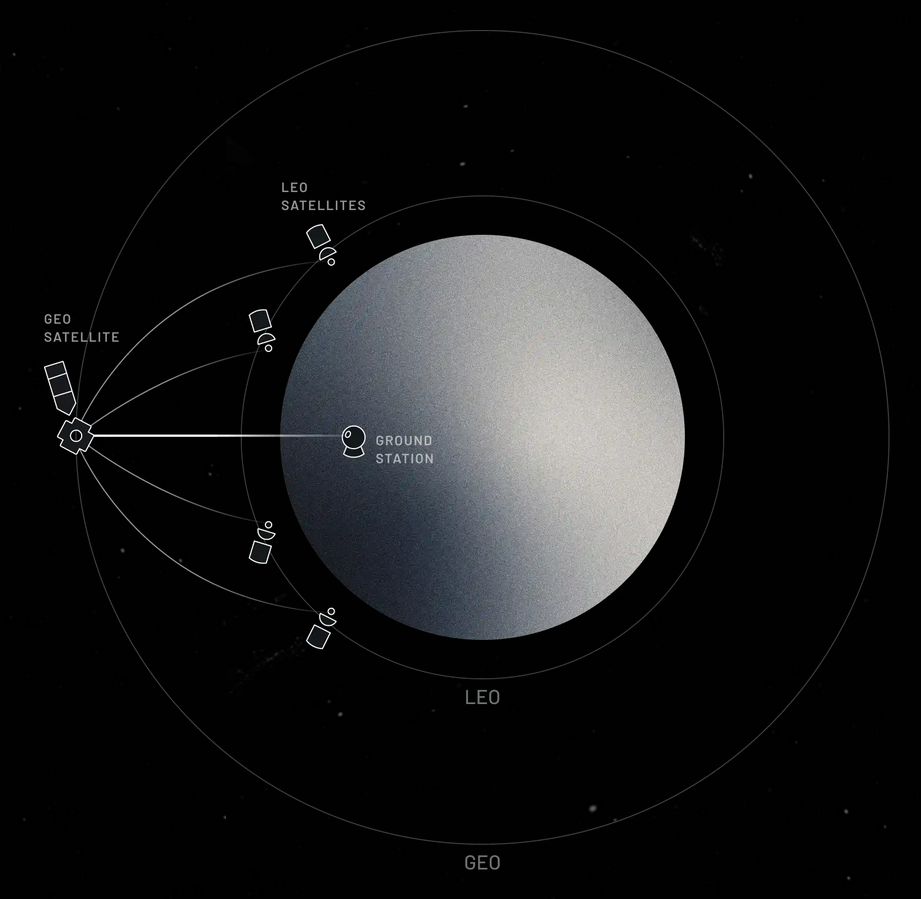
\includegraphics[width=0.8\textwidth]{./Figures/propuesta_skyloom.png}
\caption{Propuesta de la empresa Skyloom Global\protect\footnotemark.}
\label{fig:propSky}
\end{figure}

\footnotetext{Imagen tomada de \url{https://www.skyloom.co/}}

El enlace óptico, que permite la transmisión y recepción de datos a una velocidad de 1 Gbps (1 \textit{Gigabit} por segundo) entre satélites, se establece mediante una terminal de comunicaciones óptica, que es el principal producto actualmente en desarrollo por la empresa. Estas terminales cuentan con un láser que trabaja sobre una longitud de onda de 1550 nm (banda C del espectro). Dicho láser es el encargado de transmitir la información propiamente dicha mediante pulsos de luz (no visible).

En líneas generales los láseres de esta longitud de onda que se encuentran en el mercado no cuentan con la potencia óptica necesaria para que en el receptor se la detecte. Esto se debe principalmente a que la distancia de espacio libre estimada entre dos satélites en LEO es de unos 4000 km \citep{WEBSITE_SKY}.

Para solucionar el problema antes mencionado se introduce a la salida del láser un amplificador dopado con erbio o EDFA (de las siglas \textit{Erbuim Doped Fiber Amplifier}). La función de este dispositivo es aumentar la potencia del láser varias veces de forma que se alcance un nivel adecuado para la transmisión.

El modelo de amplificador utilizado por la empresa cuenta con un conector que provee una interfaz electrónica para poder controlar su funcionamiento. Esta interfaz cuenta con distintas señales y buses de comunicación que se explican con mayor detalle en la sección \ref{sec:intAmp}.

Este amplificador formará parte de la terminal de comunicaciones y estará sometido a intensivas pruebas de funcionamiento y rendimiento durante la etapa de investigación y desarrollo. Para esto es indispensable contar con una herramienta que brinde a los ingenieros a cargo de estas la posibilidad de utilizar el amplificador de forma aislada, es decir, sin tener que usar hardware de vuelo\footnote{El término \textit{de vuelo} se refiere a todo hardware que formará parte de la terminal} adicional.

En la figura \ref{fig:bloquesProy} se puede ver un esquema de uso del dispositivo junto con las conexiones con el hardware externo.

\begin{figure}[H]
\centering
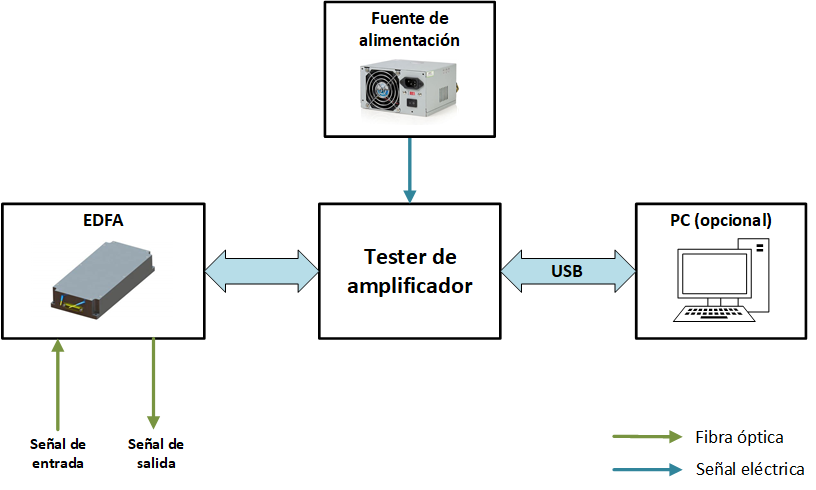
\includegraphics[width=0.85\textwidth]{./Figures/bloquesProy.png}
\caption{Esquema de uso y conexionado del sistema.}
\label{fig:bloquesProy}
\end{figure}

El dispositivo cuenta con tres conexiones externas: la interfaz con el amplificador, la conexión a la fuente de alimentación y un puerto USB.

La interfaz con el EDFA permite controlarlo y consultar diversos parámetros de funcionamiento a través de las señales presentes en el conector. La fuente de alimentación se encarga de energizar el tester y el EDFA. Y por último, la conexión USB permite controlar el amplificador del mismo modo que en el tester, por lo que el uso de la PC es opcional. Para poder hacer esto, sobre esta debe correr un software que permita establecer una comunicación.

%----------------------------------------------------------------------------------------

\section{Producto existente}

Actualmente el fabricante del amplificador posee a la venta una placa electrónica capaz de conectarse a un EDFA y proveer ciertas funcionalidades similares. La empresa ha hecho uso de ella en el pasado pero luego pasó a descartarla debido a tres problemas mayores:

\begin{itemize}
\item No permite el uso de todas las señales presentes en el conector del amplificador
\item Tiene una alta tasa de fallas
\item Su costo es muy elevado en relación a sus prestaciones
\end{itemize}

Lo expuesto anteriormente es uno de los principales motivos que dieron origen a la necesidad de contar con el sistema propuesto en este trabajo.

%----------------------------------------------------------------------------------------

\section{Objetivos y alcance}

El objetivo principal de este trabajo fue el desarrollo de un dispositivo capaz de controlar y realizar mediciones sobre un amplificador de fibra óptica. Las tareas contempladas fueron:

\begin{itemize}
\item Diseño y construcción de un prototipo funcional del dispositivo
\item Diseño e implementación del firmware del dispositivo
\item Diseño de los bancos de prueba y ensayos
\item Simulación del funcionamiento del hardware mediante software
\item Documentación de diseño y manual de uso
\end{itemize}

Los puntos del desarrollo que no se contemplaron en el trabajo fueron:

\begin{itemize}
\item Diseño y construcción de la versión final del dispositivo
\item Especificación de las pruebas a ejecutar sobre el amplificador óptico utilizando el dispositivo
\item Fabricación del PCB del dispositivo
\item Procesamiento e interpretación de los valores de los parámetros del EDFA
\item Diseño y construcción de la fuente de alimentación externa
\item Diseño e implementación del software a ejecutarse en la PC
\end{itemize}


%----------------------------------------------------------------------------------------

\chapter{Introducción específica} % Main chapter title

\label{Chapter2}

%----------------------------------------------------------------------------------------
%	Chapter 2
%----------------------------------------------------------------------------------------

Este capítulo lista los requerimientos y en base a ellos presenta y describe los componentes internos del sistema desarrollado, junto con las tecnologías y recursos de software utilizados para su implementación. 

\section{Funcionamiento de un amplificador óptico}
\label{sec:funcAmp}

\section{Interfaz del amplificador óptico}
\label{sec:intAmp}

Como se mencionó en la sección anterior, para poder controlarlo el EDFA cuenta con un conector de 25 pines tipo microD-25. Este conector contiene varios grupos de señales con distintas funciones. La tabla \ref{tab:señalesConector} lista cada una de las señales de la interfaz, junto con los detalles de su dirección, tipo y función.

\begin{table}[H]
	\centering
	\caption{Señales de la interfaz del EDFA}
	\begin{tabular}{l c p{1.5cm} p{5cm}}
		\toprule
		\textbf{Nombre de la señal}	& \textbf{Dirección}	& \textbf{Tipo} & \textbf{Función} \\
		\midrule
		5V 					& Entrada	& Potencia			& Entrada de alimentación del EDFA \\		
		PGND				& Salida	& Potencia  		& Retorno de alimentación (potencia) \\
		GND					& Salida	& Tierra digital  	& Retorno de alimentación (digital) \\
		IN\_POW				& Salida	& Analógica 		& Indica el nivel de potencia óptica de entrada \\
		OUT\_POW			& Salida	& Analógica 		& Indica el nivel de potencia óptica de salida \\
		CASE\_TEMP\_ALARM	& Salida	& Digital 			& Alarma de temperatura de la carcasa del EDFA \\
		PUMP\_BIAS\_ALARM	& Salida	& Digital 			& Alarma de la bomba de polarización \\
		OUT\_POW\_ALARM		& Salida	& Digital 			& Alarma de nivel de potencia de salida \\
		IN\_POW\_ALARM		& Salida	& Digital 			& Alarma de nivel de potencia de entrada \\
		EN/DIS				& Entrada	& Digital 			& Habilitación del amplificador \\
		RESET\_uC			& Entrada	& Digital 			& Reset del microcontrolador del EDFA \\
		OUT\_POW\_MUTE		& Entrada	& Digital 			& Habilitación de la salida óptica \\
		UART\_TX			& Salida	& Digital 			& Transmisor del UART interno del EDFA \\
		UART\_RX			& Entrada	& Digital 			& Receptor del UART interno del EDFA \\
		\bottomrule
		\hline
	\end{tabular}
	\label{tab:señalesConector}
\end{table}

A continuación, se provee una breve explicación de cada grupo de señales:
\begin{itemize}
\item Alimentación: tiene separada la tierra en digital, para la lógica y la comunicación, y la de potencia para la amplificación de la señal óptica
\item Señales analógicas: indican el nivel de potencia óptica de entrada y salida del EDFA
\item Alarmas: Mediante un estado en alto indican si ocurrió alguno de los eventos que requieren la atención del usuario
\item Señales de control: Controlan el funcionamiento de ciertos componentes del amplificador
\item Comunicación UART: Permite el envío de comandos al EDFA y la consulta de valores de parámetros internos como temperaturas, potencias, ganancias, etc.
\end{itemize}

\section{Requerimientos}

Los requerimientos fueron determinados en conjunto con la empresa en base a las funcionalidades y prestaciones con las que debe contar el sistema. Como la lista es muy extensa, se listan a continuación solamente algunos de los principales:

\renewcommand{\labelenumii}{\arabic{enumi}.\arabic{enumii}}

\begin{enumerate}

\item Encendido y apagado del EDFA
	\begin{enumerate}
	\item El software debe apagar la salida óptica del dispositivo 			EDFA bajo prueba cuando se detecte la activación de alguna de las 		alarmas.
	\item Mediante la función táctil de la pantalla LCD el usuario 			debe poder prender y apagar la alimentación del dispositivo EDFA 		bajo prueba y su salida óptica.
	\item El software debe cortar la alimentación del dispositivo EDFA 	bajo prueba cuando se detecte que la corriente supera el valor 			previamente definido.
	\item El software debe medir y mostrar en pantalla los valores de 		tensión de alimentación y consumo de corriente del dispositivo 			EDFA bajo prueba mediante las señales analógicas de entrada 			provenientes de los respectivos monitores, con una precisión no 		menor al 10\% (máximo desvío con respecto al valor real). Este 			valor debe ser de una cifra significativa para la parte entera y 		dos para la decimal.
	\end{enumerate}

\item Pantalla LCD
	\begin{enumerate}
	\item El software debe actualizar la imagen de la pantalla cada 		medio segundo (2 cuadros por segundo).
	\item La pantalla deberá indicar el estado de la salida óptica del 	dispositivo EDFA bajo prueba y el del relé de alimentación.
	\item Mediante la función táctil de la pantalla LCD el usuario 			debe poder cambiar el valor para el cual se detecta una 				sobrecorriente. El rango válido para este valor debe ser de 0 A a 		3 A, siendo la parte decimal de dos cifras significativas.
	\end{enumerate}
	
\item Entradas y salidas del EDFA
	\begin{enumerate}
	\item El software deberá mostrar en la pantalla los estados de todas las señales digitales de entrada y salida del dispositivo EDFA bajo prueba.
	\end{enumerate}

\item Requisitos de rendimiento
	\begin{enumerate}
	\item La apertura del relé de alimentación del dispositivo EDFA 		bajo prueba deberá efectuarse en un tiempo menor a 50 ms luego de 		detectarse una sobrecorriente o una caída de la tensión de 				alimentación.
	\item El apagado de la salida óptica del dispositivo EDFA bajo 			prueba deberá efectuarse en un tiempo menor a 100 ms luego de 			detectarse la activación de una alarma.
	\end{enumerate}
	
\end{enumerate}

\section{Componentes del sistema}

Los componentes de hardware que forman parte de los bloques del sistema presentado en la sección anterior fueron seleccionados con el objetivo de cumplir con los requisitos y a su vez utilizar la menor cantidad posible. Así se logra mantener al sistema simple, con poca probabilidad de fallas y fácil de usar y probar.

\subsection{Microcontrolador}

El modelo de microcontrolador utilizado es el STM32F429, del fabricante ST y con arquitectura de procesador ARM Cortex-M.

La principal razón por la que se decidió utilizar este modelo es porque es el que se encuentra integrado en la placa de desarrollo Nucleo-144, utilizada durante la cursada de la Especialización. Algunas de sus características mas relevantes para esta aplicación son \citep{STM32F429}:

\begin{itemize}
\item Núcleo CPU Arm® Cortex®-M4 de 32 bit con unidad de punto flotante, frecuencia hasta 180 MHz, unidad de protección de memoria e instrucciones DSP
\item Memoria Flash de hasta 2 MB
\item Interfaces de comunicación:
	\begin{itemize}
	\item 3 interfaces I2C
	\item 4 UART/USART (hasta 11.25 Mbit/s)
	\item 6 interfaces SPI (hasta 45 Mbit/s)
	\end{itemize}
\item Hasta 168 puertos de entrada/salida con interrupción
\item 3 conversores ADC de 12 bit de resolución y 2.4 MSPS. Hasta 24 canales
\item DMA de propósito general con FIFO y soporte de ráfaga
\item Interfaces SWD y JTAG para depuración
\item Hasta 12 \textit{timers} de 16 bits con IC/OC y PWM
\end{itemize}

La alta velocidad de reloj, la gran capacidad de memoria Flash y la gran cantidad de periféricos disponibles hacen a este modelo ideal para la ejecución de un RTOS.

La principal ventaja de utilizar la placa de desarrollo Nucleo-144 es que esta ya trae incorporada la interfaz de programación y depuración ST-LINK/V2 \citep{NUCLEO144}.

\subsection{Monitor de corriente}

El circuito integrado elegido para efectuar la medición de corriente de alimentación del amplificador mientras este se encuentra en funcionamiento es el INA301A3. Sus principales características son:

\begin{itemize}
\item Alto rango de tensión de modo común (0 V a 36 V)
\item Salida analógica y a comparador
\item Máxima tensión de \textit{offset} de salida: 35 uV
\item Máximo error de ganancia: 0.1%
\item Ganancia del amplificador: 100 V/V
\item Nivel de alerta programable mediante un resistor
\item Tiempo total de respuesta de la alerta: 1 us
\end{itemize}

Este chip provee en uno de sus pines una tensión analógica proporcional a la corriente que se está midiendo. Asimismo, cuenta con una salida digital que se activa cuando la corriente medida alcanza cierto nivel establecido mediante un resistor (pin ALERT) \citep{INA301}.

\subsection{Pantalla táctil LCD}

El modelo del módulo de la pantalla LCD utilizada en el trabajo es MSP2807 y es una solución integrada, es decir, cuenta con toda la electrónica necesaria para poder hacer uso de la pantalla en su totalidad. Para esto cuenta con dos circuitos integrados: el controlador del display de la pantalla (lo que permite dibujar en ella) y el controlador de la función táctil (lo que permite detectar cuando se la toca). En la figura \ref{fig:pantLCD} se puede ver una imagen de la pantalla.

\begin{figure}[H]
\centering
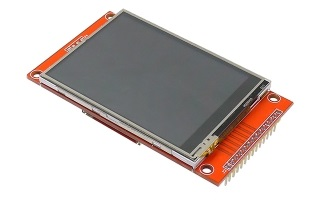
\includegraphics[width=0.7\textwidth]{./Figures/pant_LCD.png}
\caption{Pantalla LCD táctil MSP2807}
\label{fig:pantLCD}
\end{figure}

En la tabla \ref{tab:caractLCD} se listan las características de la pantalla.

\begin{table}[H]
	\centering
	\caption{Características de la pantalla LCD}
	\begin{tabular}{l c}
		\toprule
		\textbf{Característica}	& \textbf{Valor} \\
		\midrule
		Color				& 65K colores RGB \\
		Tamaño				& 2.8 pulgadas (7.11 cm) \\
		Tipo de pantalla	& TFT \\
		Resolución			& 320x240 pixeles \\
		Área activa			& 43.2x57.6 mm \\
		Tensión de alimentación		& 3.3 V - 5 V \\
		Nivel lógico de I/O			& 3.3 V (TTL) \\		
		\bottomrule
		\hline
	\end{tabular}
	\label{tab:caractLCD}
\end{table}

El controlador del display tiene una interfaz SPI para el envío de los datos y además una señal denominada DC/RS para indicar si lo que está enviando el maestro es un dato o un registro interno del chip. También consta de una señal de reset para borrar todo el contenido del display.

El controlador de la función táctil también tiene un bus SPI y una señal adicional de interrupción denominada T\_IRQ que indica cuando el display está siendo tocado \citep{MSP2807}.

\section{Recursos de software}

Para el firmware del microcontrolador se usaron distintas herramientas que permitieron el desarrollo de una estructura de software jerárquita, simple y eficaz.

\subsection{Sistema operativo de tiempo real FreeRTOS}

FreeRTOS es un sistema operativo de tiempo real o RTOS (de \textit{Real Time Operating System}) para microcontroladores o pequeños microprocesadores, diseñado para ocupar poco espacio, ser confiable y fácil de usar. Está escrito en C para que sea fácil de mantener y trasladar a nuevos dispositivos.

FreeRTOS provee recursos que facilitan la ejecución de aplicaciones sobre el sistema operativo como tareas, semáforos, \textit{mutexes}, temporizadores por software, colas y gestores de memoria dinámica \citep{WEBSITE:1}.

Si se separa el firmware en capas desde la mas baja (hardware) hasta la mas alta (aplicación de usuario) el lugar que ocupa FreeRTOS se ubica por arriba de los drivers provistos por el fabricante, brindando una capa de abstracción de mayor nivel. De esta forma, el sistema operativo actúa como puente entre las capas mas bajas y las mas altas, gestionando los recursos de hardware de forma automática y brindando servicios a la capa de aplicación.

En la figura \ref{fig:capas} se puede ver la estructura de capas del firmware con FreeRTOS incluída.

\begin{figure}[H]
\centering
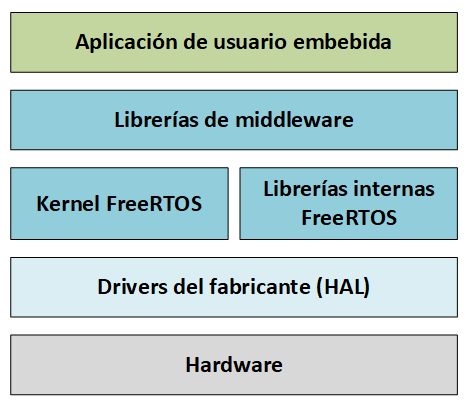
\includegraphics[width=0.65\textwidth]{./Figures/capas.png}
\caption{Estructura de capas con FreeRTOS}
\label{fig:capas}
\end{figure}

Uno de las ventajas principales de usar FreeRTOS es la posibilidad de ejecutar varias tareas o \textit{tasks} en forma simultánea tal como lo hace un sistema operativo cualquiera. Un \textit{scheduler} gestiona la ejecución de cada una de forma individual y con su propio contexto (\textit{stack} y variables). Esto permite estructurar la aplicación separándola en tareas independientes pero sincronizadas \citep{WEBSITE:FREERTOS}.

\subsection{Capa de abstracción de hardware (HAL)}

\section{Periféricos utilizados}

A excepción del monitor de corriente, el resto de los periféricos utilizados ya se encuentran integrados en el chip del microcontrolador, por lo que no hubo que agregar ningún hardware adicional y para poder utilizarlos solo hizo falta leer las hojas de datos. De todas formas, en esta sección se provee una breve descripción de cada uno.

\subsection{Conversor analógico-digital (ADC)}

Un conversor analógico-digital o ADC (de \textit{Analog-to-Digital Converter}) es un dispositivo que convierte una señal eléctrica analógica proveniente, por ejemplo, de un sensor a una señal digital. La principal ventaja de esta conversión es que su valor puede ser almacenado en un sistema digital, por lo que estará representada por un número binario.

La señal pasa de ser continua en el tiempo y contínua en amplitud a discreta en el tiempo y discreta en amplitud. Esto quiere decir que la señal analógica podría tomar cualquier valor en cualquier instante. En cambio cuando es convertida la señal se encuentra cuantizada, es decir, podrá tomar solamente determinados valores que dependen de la cantidad de bits del ADC y del fondo de escala (resolución).

Esto hace que no se puedan representar todos los valores que se miden, y cada muestra tomada estará truncada al valor mas cercano representable. Este error introducido en la medición se denomina error de cuantización. A modo de ejemplo, en la figura \ref{fig:muestreoADC} se muestra un ejemplo de una conversión analógica-digital con un ADC de 3 bits. La señal de entrada (en rojo) es muestreada a intervalos constantes y la señal resultante (en azul) está cuantizada.

\begin{figure}[H]
\centering
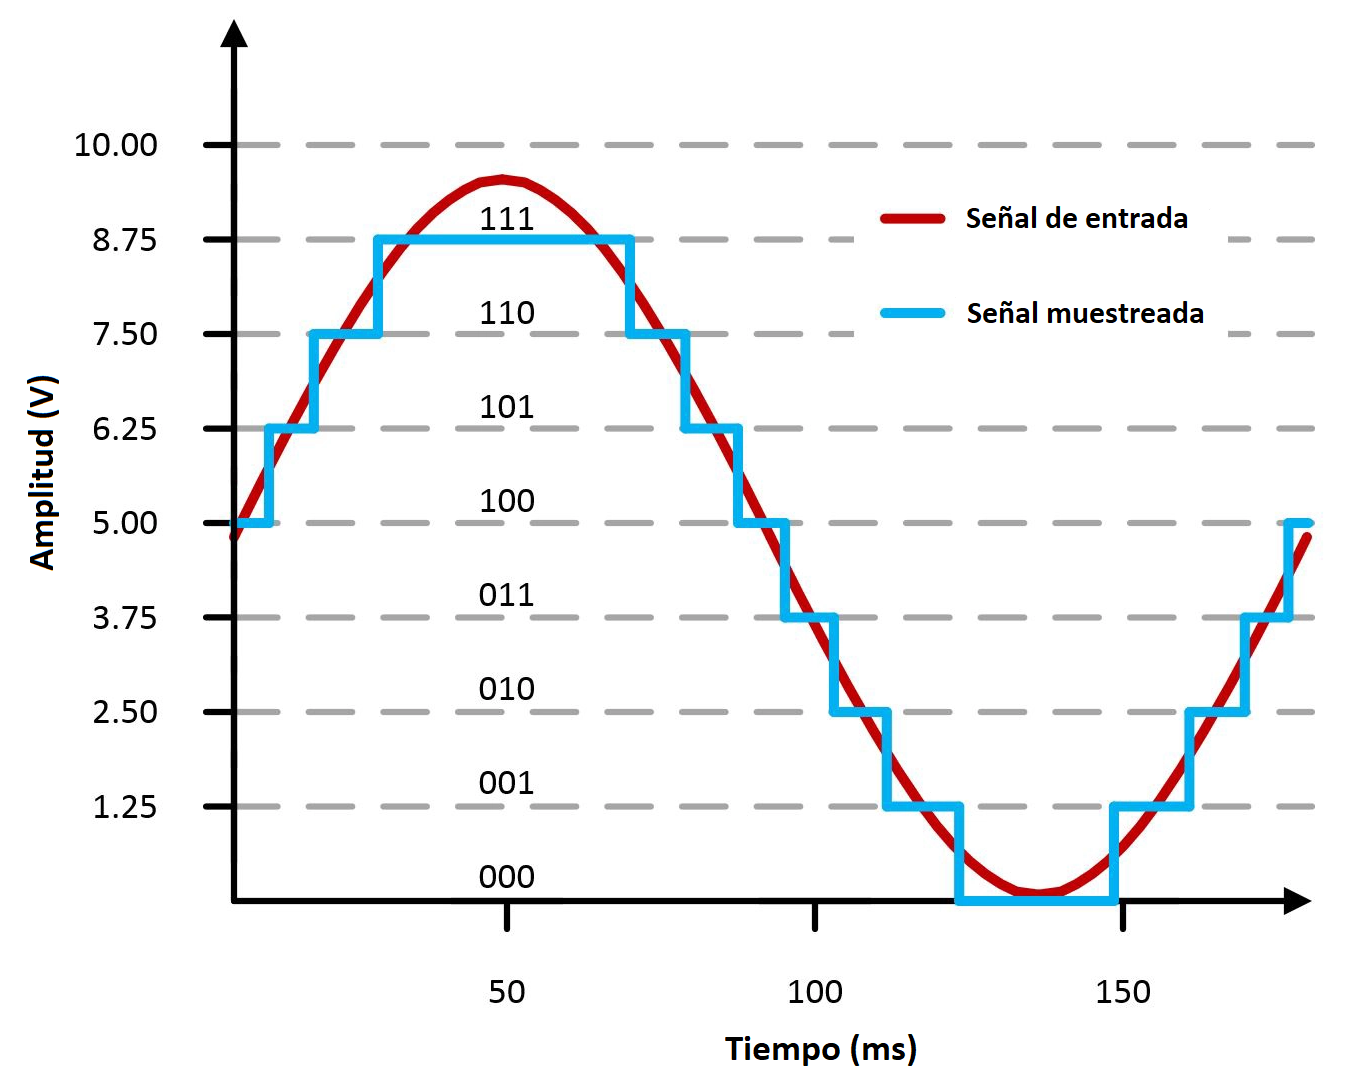
\includegraphics[width=0.65\textwidth]{./Figures/muestreo.png}
\caption{Conversión de una señal con un ADC de 3 bits}
\label{fig:muestreoADC}
\end{figure}

De la figura \ref{fig:muestreoADC} se puede ver que mientras mas bits de resolución tenga el ADC, se van a poder tomar valores mas cercanos al medido y por lo tanto tener una mejor representación de la señal.

Esto impacta directamente en el parámetro de relación señal-ruido que, junto con el ancho de banda (velocidad de muestreo), es uno de los parámetros con los que se caracteriza el rendimiento de un ADC \citep{WEBSITE:2}.

\subsection{Universal Asynchronous Receiver Transmitter (UART)}

Un UART es un dispositivo utilizado para establecer una comunicación serie asíncrona, con formato de datos y velocidad de transmisión configurables. Consta solo de dos señales que conectan dos dispositivos de forma bidireccional: una para la transmisión y otra para la recepción, comunmente llamdas TX y RX respectivamente.

La forma de transmisión de datos del protocolo tiene una estructura específica. Por cada dato que se transmite (cuyo ancho puede variar entre 5 y 9 bits), se transmiten además bits adicionales de comienzo y fin de trama (\textit{Start} y \textit{Stop}) y, opcionalmente, los de paridad para la detección de errores. En la figura \ref{fig:transUART} se puede ver la composición de una trama completa.

\begin{figure}[H]
\centering
\includegraphics[width=0.9\textwidth]{./Figures/UART_frame.png}
\caption{Trama de transmisión UART}
\label{fig:transUART}
\end{figure}

Los bits de \textit{Start} y \textit{Stop} son para indicarle al receptor cuando debe comenzar y cuando parar de tomar los datos transmitidos. También sirve para realizar una sincronización de los relojes del transmisor y del receptor. Como el protocolo es asíncrono, es decir, no transmite el reloj en ninguna de sus líneas, los relojes internos de ambos deben estar en fase.

El estado \textit{Idle} de la línea es el estado inactivo, es decir, el estado de reposo cuando no se encuentra transmitiendo \citep{WEBSITE:3}.

\subsection{Serial Peripheral Interface (SPI)}

%En la figura \ref{fig:transSPI}

%\begin{figure}[H]
%\centering
%\includegraphics[width=0.85\textwidth]{./Figures/.png}
%\caption{Transacción SPI}
%\label{fig:transSPI}
%\end{figure} 
\chapter{Diseño e implementación} % Main chapter title

\label{Chapter3} % Change X to a consecutive number; for referencing this chapter elsewhere, use \ref{ChapterX}

\definecolor{mygreen}{rgb}{0,0.6,0}
\definecolor{mygray}{rgb}{0.5,0.5,0.5}
\definecolor{mymauve}{rgb}{0.58,0,0.82}

%%%%%%%%%%%%%%%%%%%%%%%%%%%%%%%%%%%%%%%%%%%%%%%%%%%%%%%%%%%%%%%%%%%%%%%%%%%%%
% parámetros para configurar el formato del código en los entornos lstlisting
%%%%%%%%%%%%%%%%%%%%%%%%%%%%%%%%%%%%%%%%%%%%%%%%%%%%%%%%%%%%%%%%%%%%%%%%%%%%%
\lstset{ %
  backgroundcolor=\color{white},   % choose the background color; you must add \usepackage{color} or \usepackage{xcolor}
  basicstyle=\footnotesize,        % the size of the fonts that are used for the code
  breakatwhitespace=false,         % sets if automatic breaks should only happen at whitespace
  breaklines=true,                 % sets automatic line breaking
  captionpos=b,                    % sets the caption-position to bottom
  commentstyle=\color{mygreen},    % comment style
  deletekeywords={...},            % if you want to delete keywords from the given language
  %escapeinside={\%*}{*)},          % if you want to add LaTeX within your code
  %extendedchars=true,              % lets you use non-ASCII characters; for 8-bits encodings only, does not work with UTF-8
  %frame=single,	                % adds a frame around the code
  keepspaces=true,                 % keeps spaces in text, useful for keeping indentation of code (possibly needs columns=flexible)
  keywordstyle=\color{blue},       % keyword style
  language=[ANSI]C,                % the language of the code
  %otherkeywords={*,...},           % if you want to add more keywords to the set
  numbers=left,                    % where to put the line-numbers; possible values are (none, left, right)
  numbersep=5pt,                   % how far the line-numbers are from the code
  numberstyle=\tiny\color{mygray}, % the style that is used for the line-numbers
  rulecolor=\color{black},         % if not set, the frame-color may be changed on line-breaks within not-black text (e.g. comments (green here))
  showspaces=false,                % show spaces everywhere adding particular underscores; it overrides 'showstringspaces'
  showstringspaces=false,          % underline spaces within strings only
  showtabs=false,                  % show tabs within strings adding particular underscores
  stepnumber=1,                    % the step between two line-numbers. If it's 1, each line will be numbered
  stringstyle=\color{mymauve},     % string literal style
  tabsize=2,	                   % sets default tabsize to 2 spaces
  title=\lstname,                  % show the filename of files included with \lstinputlisting; also try caption instead of title
  morecomment=[s]{/*}{*/}
}


%----------------------------------------------------------------------------------------
%	SECTION 1
%----------------------------------------------------------------------------------------
\section{Dispositivo implementado}
 
La idea de esta sección es resaltar los problemas encontrados, los criterios utilizados y la justificación de las decisiones que se hayan tomado.

Se puede agregar código o pseudocódigo dentro de un entorno lstlisting con el siguiente código:

\begin{verbatim}
\begin{lstlisting}[caption= "un epígrafe descriptivo"]
	las líneas de código irían aquí...
\end{lstlisting}
\end{verbatim}

A modo de ejemplo:

\begin{lstlisting}[label=cod:vControl,caption=Pseudocódigo del lazo principal de control.]  % Start your code-block

#define MAX_SENSOR_NUMBER 3
#define MAX_ALARM_NUMBER  6
#define MAX_ACTUATOR_NUMBER 6

uint32_t sensorValue[MAX_SENSOR_NUMBER];		
FunctionalState alarmControl[MAX_ALARM_NUMBER];	//ENABLE or DISABLE
state_t alarmState[MAX_ALARM_NUMBER];						//ON or OFF
state_t actuatorState[MAX_ACTUATOR_NUMBER];			//ON or OFF

void vControl() {

	initGlobalVariables();
	
	period = 500 ms;
		
	while(1) {

		ticks = xTaskGetTickCount();
		
		updateSensors();
		
		updateAlarms();
		
		controlActuators();
		
		vTaskDelayUntil(&ticks, period);
	}
}
\end{lstlisting}

\section{Arquitectura de hardware}

\subsection{Monitor de corriente}

\section{Arquitectura de software}

\subsection{Maquina de estados}

\subsection{Capa de abstraccion de la placa}



% Chapter Template

\chapter{Ensayos y resultados} % Main chapter title

\label{Chapter4} % Change X to a consecutive number; for referencing this chapter elsewhere, use \ref{ChapterX}

%----------------------------------------------------------------------------------------
%	CHAPTER 4
%----------------------------------------------------------------------------------------

En este capítulo se explica cómo se llevaron a cabo las pruebas de validación de hardware y software a las que fue sometido el dispositivo, los bancos de ensayos, instrumentos utilizados y los resultados obtenidos.

\section{Instrumental utilizado}

Para poder ejecutar las pruebas de integración de hardware y software se requirió del uso de una variedad de instrumentos y componentes en los bancos de ensayos. La tabla \ref{tab:instrumentos} lista los detalles de cada uno de ellos.

\begin{table}[H]
	\centering
	\caption{Lista de instrumental utilizado.}
	\begin{tabular}{p{3cm} c p{6cm}}
		\toprule
		\textbf{Item} & \textbf{Modelo} & \textbf{Descripción} \\
		\midrule
		Multímetro			& UNI-T UT61A		& Multímetro digital autorango de alta precisión. \\
		Fuente de tensión	& KM GP-300ATX		& Fuente de computadora de 400 W. \\
		Resistencia de potencia variable		& AVT05006E25R00KE	& Resistencia de potencia de alambre bobinado de 25 Ohm / 50 W. \\
		Potenciómetro							& 3590S-1-201L & Potenciómetro de 200 Ohm / 2 W y 10 vueltas para panel. \\
		Conversor USB a UART					& EM7-6043		& Conversor USB a serie TTL CH-340. \\
		Cables varios							& - 			& Cables dupont y unipolar de 2,5 mm2. \\
		PC										& -				& Computadora de escritorio con software PuTTY (cliente de terminal). \\
		\bottomrule
		\hline
	\end{tabular}
	\label{tab:instrumentos}
\end{table}

En el apéndice \ref{AppendixB} se puede ver una foto del banco de ensayos completo con todos los instrumentos y hardware utilizado.

\section{Pruebas de hardware}
\label{sec:pruebasHW}

Para validar el funcionamiento del hardware, basta con medir continuidad o niveles de tensión en ciertos puntos de la placa. Por esta razón, se omite especificar las pruebas a excepción de las del monitor de corriente, ya que es el único caso en el que es necesario realizar mediciones.

\subsection{Prueba del monitor de corriente}
\label{sec:monCorr}

En el circuito del monitor de corriente lo que se desea verificar es que a la salida del amplificador se obtenga una tensión proporcional al valor de corriente que circula. La constante de conversión surge de multiplicar el valor de la resistencia de sensado (10 mOhm) por la constante de amplificación del circuito integrado (100 V/V), lo que resulta en un valor de 1 V/A. Por lo tanto, la conversión entre corriente y tensión es unitaria.

Para realizar las mediciones se conecta la entrada de tensión a la fuente de 5 V, una resistencia de potencia en la salida de tensión y se varía su valor de forma de hacer circular desde 0 A hasta aproximadamente 3,3 A.

Con los datos obtenidos se calcula para cada medición el error porcentual con respecto al valor teórico de la constante de conversión. En la figura \ref{fig:testMonCorr} se pueden ver los valores computados para distintos valores de corriente en la carga.

\begin{figure}[H]
\centering
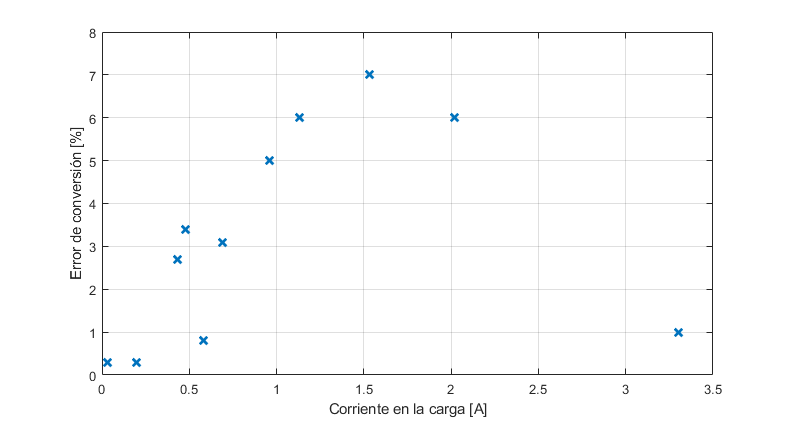
\includegraphics[width=0.9\textwidth]{./Figures/testMonCorr.png}
\caption{Error porcentual de la constante de conversión de corriente.}
\label{fig:testMonCorr}
\end{figure}

Del gráfico se observa que en este rango se tiene un error de medición máximo del 7 \% y un valor promedio aproximado del 3,23 \% respecto del valor real.

Esta diferencia entre el valor de la constante medida y el teórico se la puede atribuir principalmente a dos efectos: la dispersión del valor de la resistencia de sensado y a la presencia de ruido en el circuito. El error de la ganancia del circuito integrado está especificado en un máximo de 0,2\% por lo que no aporta variaciones significativas.

\section{Pruebas de firmware}
\label{sec:pruebasFW}

Las pruebas de firmware tienen como finalidad validar el funcionamiento individual de una biblioteca o una parte en particular del código desarrollado. Para ello, en algunos casos lo que se hace es directamente mostrar funcionalidades específicas del programa funcionando, como por ejemplo en el driver de la pantalla LCD y de la consola de control.

\subsection{Prueba del monitor de tensión}

Para el monitor de tensión y el monitor de corriente (siguiente subsección) se desea verificar que las mediciones se realizan con un error menor al especificado en el requerimiento 1.4, en la sección \ref{sec:reqs}.

Para realizar las mediciones se conecta la entrada de tensión a una fuente variable y se lee directamente el valor medido que muestra la pantalla LCD. Se toman valores en el rango entre 0 V y 5 V en pasos aproximados de 0,5 V.

Con el valor de tensión de entrada y el medido por la placa se computa el error para cada medición (con respecto al de tensión de entrada). En la figura \ref{fig:testMonTens} se pueden ver los valores computados para los distintos valores de tensión de entrada.

\begin{figure}[H]
\centering
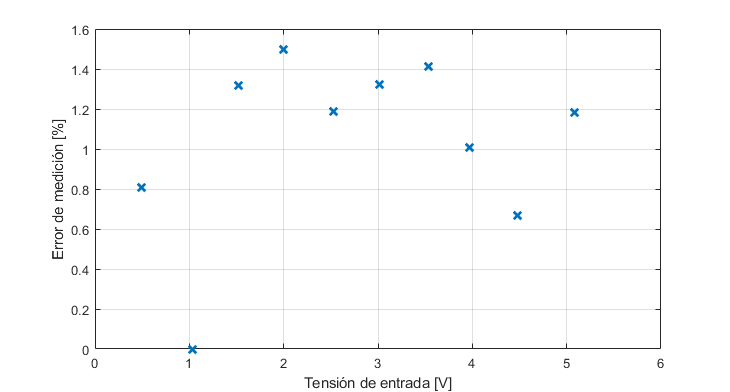
\includegraphics[width=0.9\textwidth]{./Figures/testMonTens.png}
\caption{Error porcentual de la medición de tensión.}
\label{fig:testMonTens}
\end{figure}

Del gráfico se observa que en este rango se tiene un error de medición máximo del 1,5 \% y un valor promedio aproximado del 1,04 \% respecto del valor real.

\subsection{Prueba del monitor de corriente}

Para esta prueba se procede de igual forma que en la subsección \ref{sec:monCorr} pero en lugar de medir la tensión de salida del monitor se toma directamente la lectura de medición de corriente de la pantalla LCD.

Con los datos obtenidos se calcula para cada medición el error porcentual con respecto al valor real de corriente de carga. En la figura \ref{fig:testMonCorr2} se pueden ver los valores computados para distintos valores de corriente en la carga.

\begin{figure}[H]
\centering
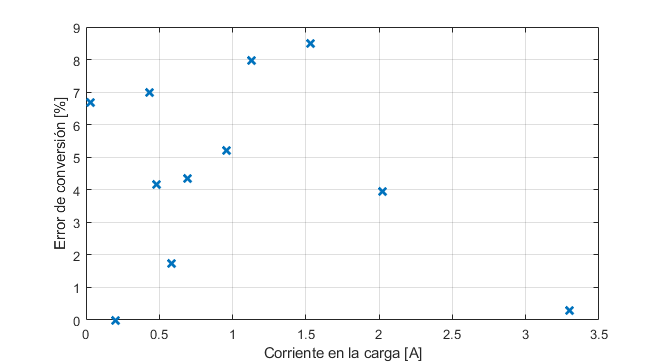
\includegraphics[width=0.9\textwidth]{./Figures/testMonCorr2.png}
\caption{Error porcentual de la medición de corriente.}
\label{fig:testMonCorr2}
\end{figure}

Observando el gráfico se desprende que en este rango se tiene un error de medición máximo del 8,5 \% y un valor promedio aproximado del 4,52 \% respecto del valor real. Estos valores resultan ligeramente mayores a los obtenidos en la sección \ref{sec:monCorr}, lo cual es de esperarse ya que durante el procesamiento digital de los datos se introduce más incerteza (debido a la resolución del ADC) y error de cálculo.

\subsection{Prueba de la pantalla LCD}

En este caso se muestra directamente el LCD durante el funcionamiento normal del programa, lo que implica no solo que la biblioteca desarrollada para la pantalla funciona, si no que los drivers del SPI sobre los que esta implementada también.

En la figura \ref{fig:testLCD} se puede ver la pantalla LCD durante el inicio del programa luego de encender la placa. Como se puede ver, contiene texto y rectángulos de distintos colores, lo que implica el uso de la mayoría de las funciones implementadas en la biblioteca.

\begin{figure}[H]
\centering
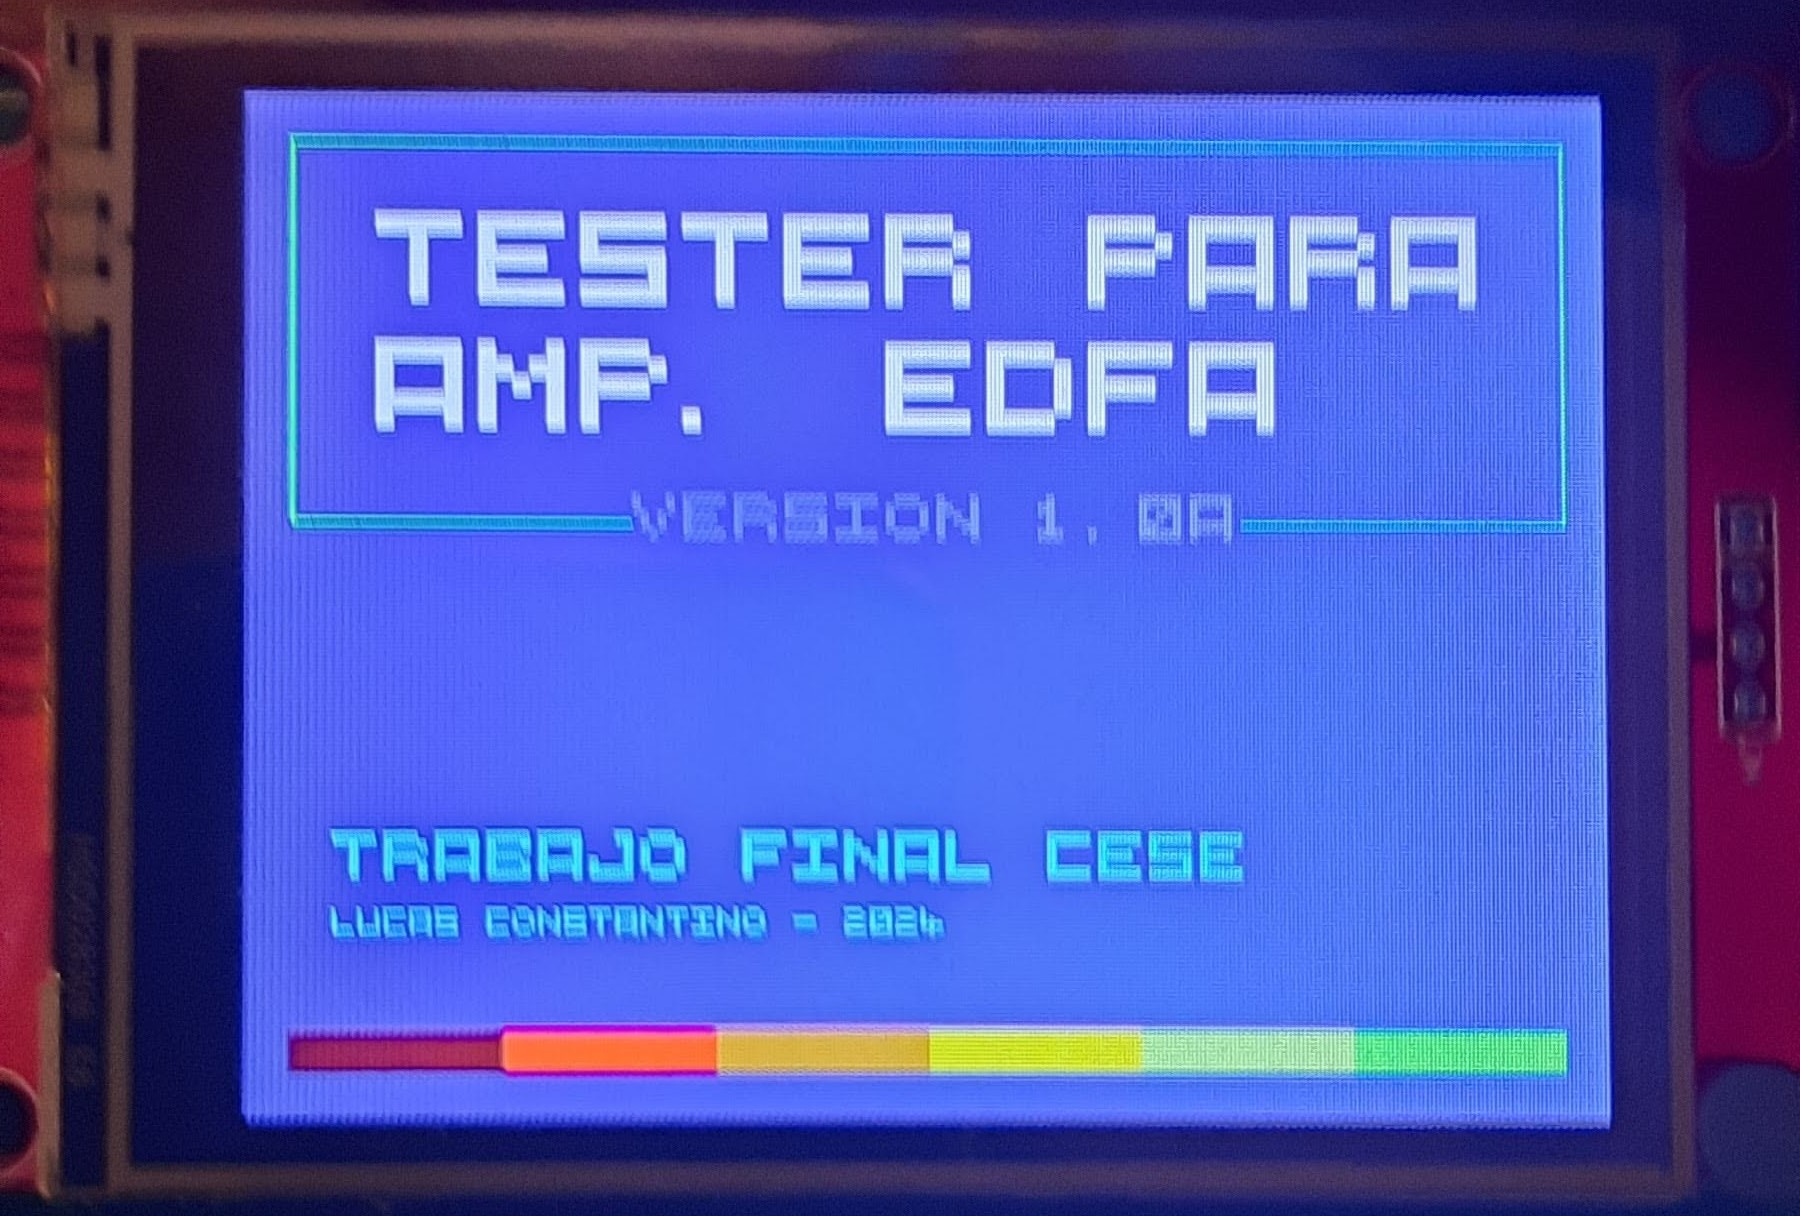
\includegraphics[width=0.8\textwidth]{./Figures/testLCD.jpg}
\caption{Pantalla LCD durante el encendido de la placa.}
\label{fig:testLCD}
\end{figure}

\subsection{Prueba de la consola de control}

La consola de control se encuentra implementada sobre el driver de la UART por lo que al validar el funcionamiento de esta también se estaría validando el del funcionamiento del driver.

Para ello lo que se hace es, mediante el emulador de puertos PuTTY, enviar mediante UART distintos comandos al microcontrolador y verificar que tienen el efecto deseado en la placa. En la figura \ref{fig:pruebaConsola} se puede ver la terminal luego de la ejecución de varios comandos.

\begin{figure}[H]
\centering
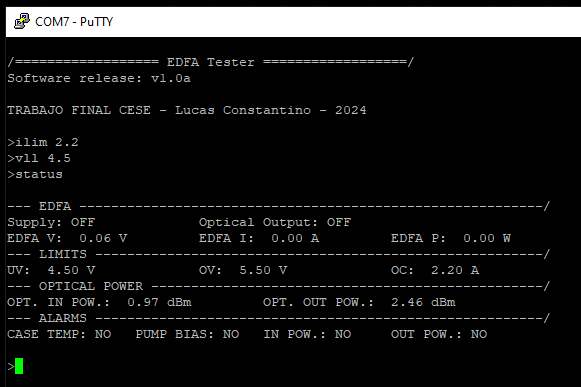
\includegraphics[width=0.9\textwidth]{./Figures/pruebaConsola.png}
\caption{Uso de la consola de control.}
\label{fig:pruebaConsola}
\end{figure}

\section{Pruebas de integración}
\label{sec:pruebasInt}

Las pruebas de integración tienen como objetivo verificar el cumplimiento de los requerimientos establecidos en el documento \citep{DOC_REQ} y mencionados en la sección \ref{sec:reqs}. Al hacer esto se valida la correcta interacción entre el hardware y el firmware, es decir, el funcionamiento del sistema como una unidad.

\subsection{Funcionamiento normal}

En la figura \ref{fig:funcNorm} se puede ver el estado de la pantalla LCD durante el funcionamiento normal, con el amplificador alimentado, su salida óptica prendida y ninguna alarma activa.

\begin{figure}[H]
\centering
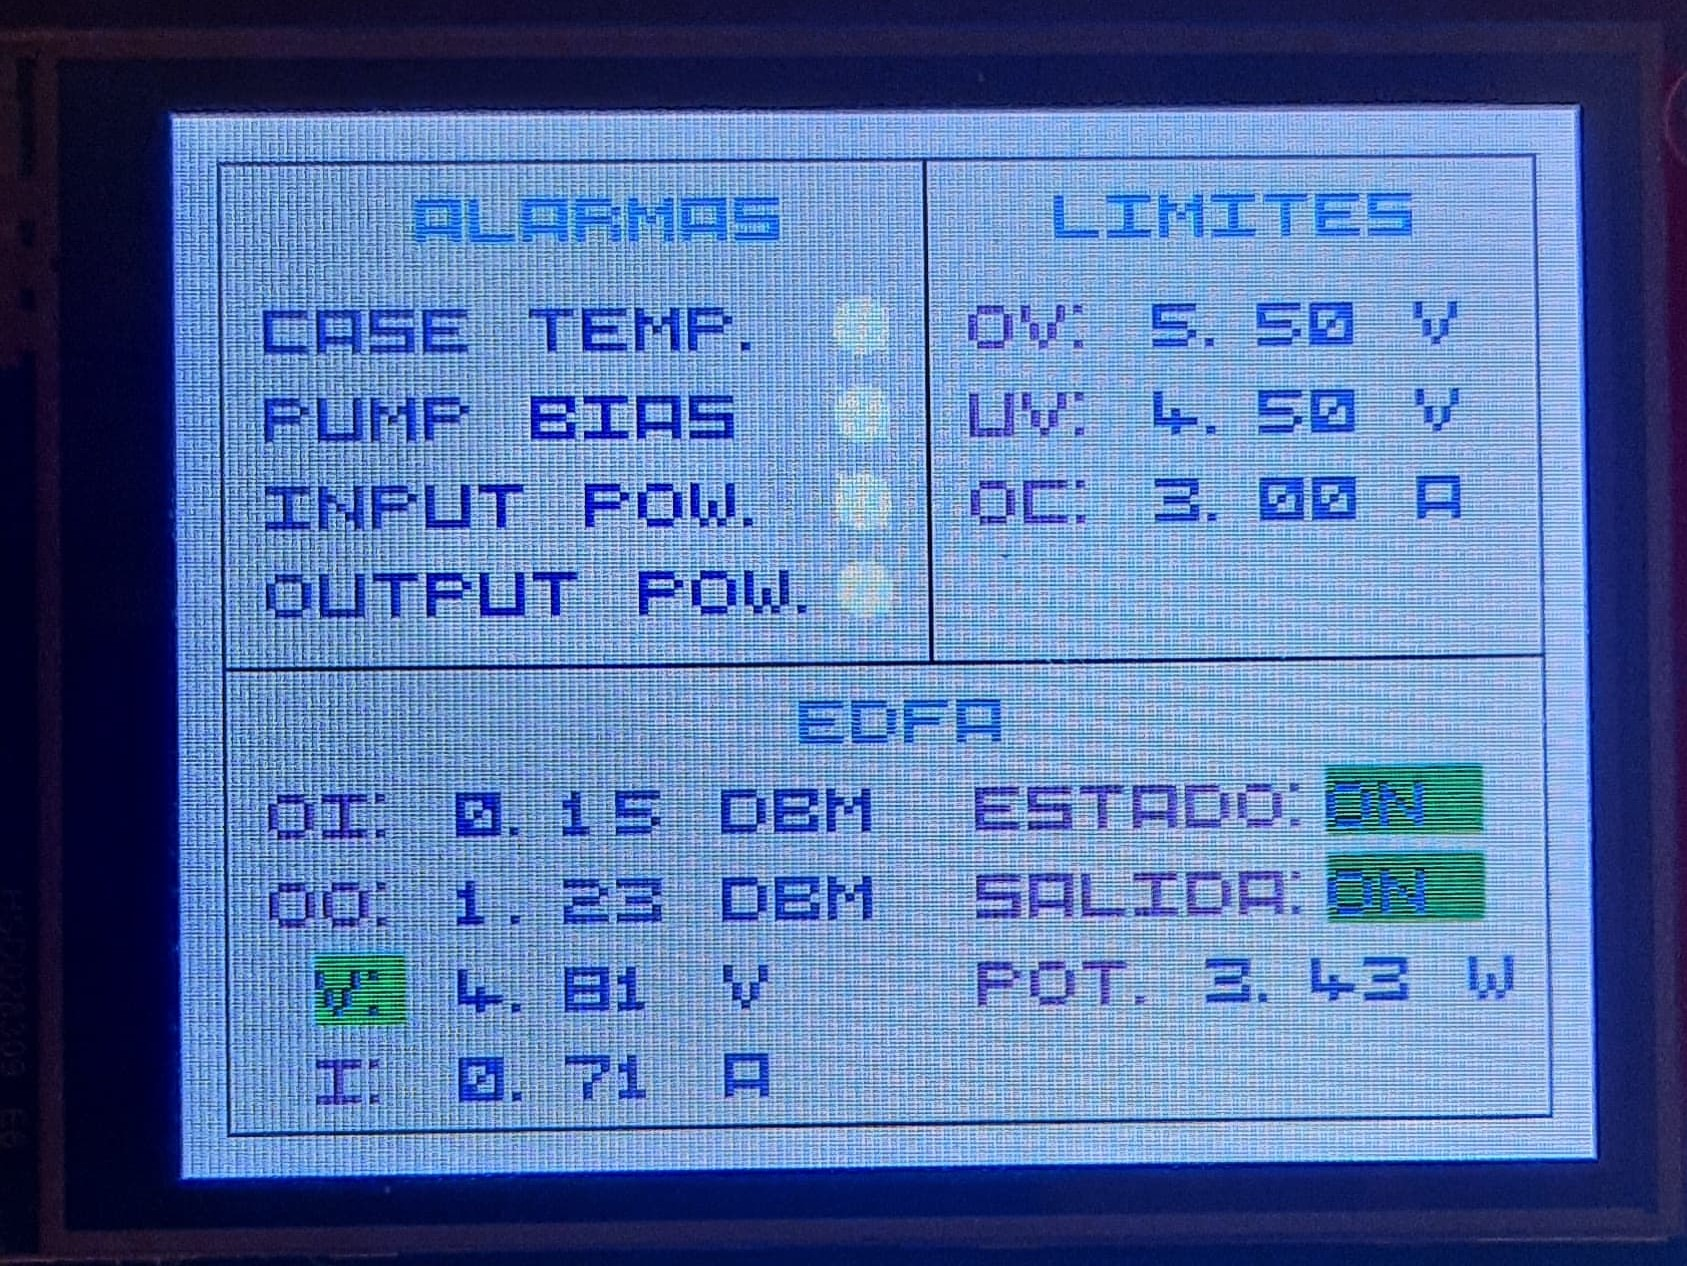
\includegraphics[width=0.75\textwidth]{./Figures/funcNorm.jpg}
\caption{Pantalla LCD durante funcionamiento normal.}
\label{fig:funcNorm}
\end{figure}

\subsection{Detección de alarmas}

Cuando alguna de las alarmas se activa mientras la salida óptica del amplificador está prendida, esta se debe apagar inmediatamente mediante la señal de control OUT POW MUTE. De lo contrario, esto podría dañar el EDFA.

En la figura \ref{fig:detecAlarm2} se puede ver la conmutación de la señal de control OUT POW MUTE (canal D1 en rojo) cuando la señal de alarma CASE TEMP se activa (canal D0 en blanco). Ambas señales son activas en nivel alto.

\begin{figure}[H]
\centering
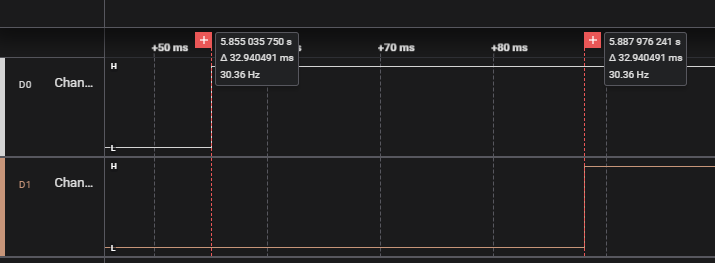
\includegraphics[width=1\textwidth]{./Figures/detecAlarm2.png}
\caption{Detección de alarma y apagado de salida óptica.}
\label{fig:detecAlarm2}
\end{figure}

En la figura anterior se puede observar que el tiempo de retardo que existe entre la detección de la alarma del EDFA y el apagado de la salida óptica es de aproximadamente 33 ms, lo cual cumple con el requerimiento 4.2 especificado en la sección \ref{sec:reqs}.

En la figura \ref{fig:detecAlarm} se puede ver el estado de la pantalla LCD luego de la detección de la alarma. El amplificador permanece alimentado pero su salida apagada.

\begin{figure}[H]
\centering
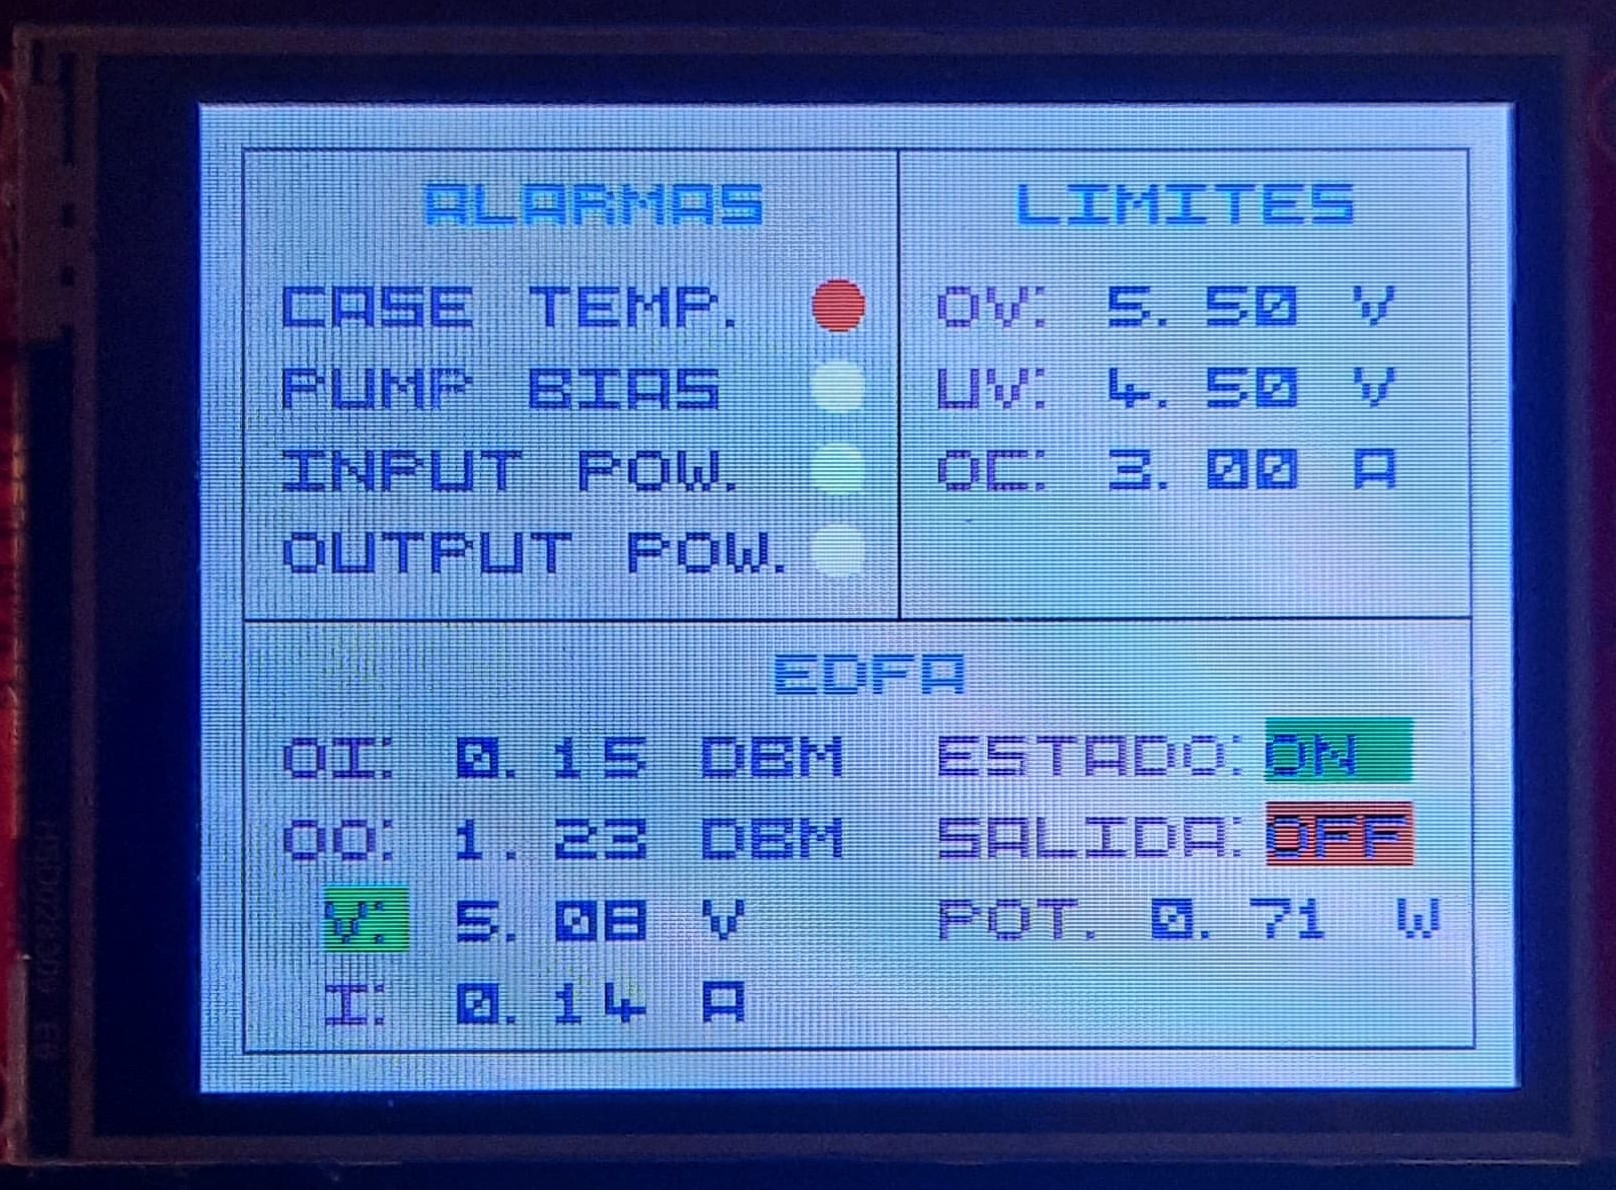
\includegraphics[width=0.75\textwidth]{./Figures/detecAlarm.jpg}
\caption{Pantalla LCD luego de detección de alarma.}
\label{fig:detecAlarm}
\end{figure}

\subsection{Detección de sobrecorriente}

Al igual que para el caso de la detección de alarmas, la detección de una sobrecorriente también debe efectuarse y procesarse rápidamente. En este caso lo que se hizo fue, asociando la señal de alarma del monitor de corriente a una interrupción en el programa, medir el retardo existente entre el momento en que se activa esta señal y se desactiva la del relé de alimentación.

En la figura \ref{fig:detecOC} se puede ver la conmutación de la señal que controla la activación del relé (canal D1 en rojo) luego de que la señal de alarma del monitor de corriente se activa (canal D0 en blanco). En este caso la alarma es activa en nivel bajo.

\begin{figure}[H]
\centering
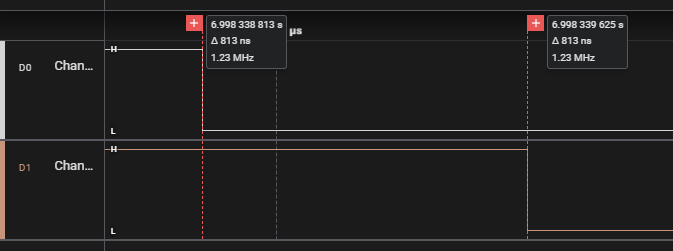
\includegraphics[width=1\textwidth]{./Figures/detecOC.png}
\caption{Detección de sobrecorriente y desconexión del EDFA.}
\label{fig:detecOC}
\end{figure}

Se puede observar que el tiempo de retardo que existe entre la detección de la sobrecorriente y la desconexión del relé es menor a 1 us, lo cual cumple holgadamente con el requerimiento 4.1 especificado en la sección \ref{sec:reqs}. 
% Chapter Template

\chapter{Conclusiones} % Main chapter title

\label{Chapter5} % Change X to a consecutive number; for referencing this chapter elsewhere, use \ref{ChapterX}


%----------------------------------------------------------------------------------------
%	Chapter 5
%----------------------------------------------------------------------------------------

El último capítulo resume los resultados alcanzados en este trabajo, el grado de cumplimiento de los requerimientos y plantea las mejoras necesarias en etapas futuras.

\section{Conclusiones generales}

En lineas generales el desarrollo del proyecto se llevó a cabo con éxito ya que, a pesar de los contratiempos encontrados, se logró:  

\begin{itemize}
\item Obtener un prototipo validado del hardware
\item Desarrollar una primera versión validada del firmware 
\item Interiorizarse en la tecnología de los EDFA y su funcionamiento
\item Como se explica en la sección \ref{sec:dispImp}, el dispositivo desarrollado no es el producto final si no una primera versión que funciona como prueba de concepto y simulador del comportamiento del amplificador. Aún así, logra cumplir con los requerimientos principales establecidos por la empresa.
\end{itemize}

\section{Trabajo futuro}

Con el objetivo de contar con un producto final apto para uso en tareas de integración e investigación y desarrollo,  se planea avanzar en varios aspectos. Entre estos se encuentran:

\begin{itemize}
\item Rediseñar el PCB a la versión final corrigiendo los errores encontrados y aplicando las modificaciones necesarias para poder conectarse a un EDFA y montarse sobre la carcasa. También se deberá incluir el microcontrolador de la placa Nucleo junto con su interfaz de programación
\item Robustecer el firmware añadiendo mas funcionalidades y corrigiendo errores
\item Una vez rediseñado el PCB, volver a validar el hardware y firmware utilizando un EDFA provisto por la empresa
\end{itemize} 

%----------------------------------------------------------------------------------------
%	CONTENIDO DE LA MEMORIA  - APÉNDICES
%----------------------------------------------------------------------------------------

\appendix % indicativo para indicarle a LaTeX los siguientes "capítulos" son apéndices

% Incluir los apéndices de la memoria como archivos separadas desde la carpeta Appendices
% Descomentar las líneas a medida que se escriben los apéndices

\begin{landscape}

% Appendix A

\chapter{Circuito esquemático completo} % Main appendix title

\label{AppendixA} % For referencing this appendix elsewhere, use \ref{AppendixA}

Write your Appendix content here.

\begin{figure}[H]
\centering
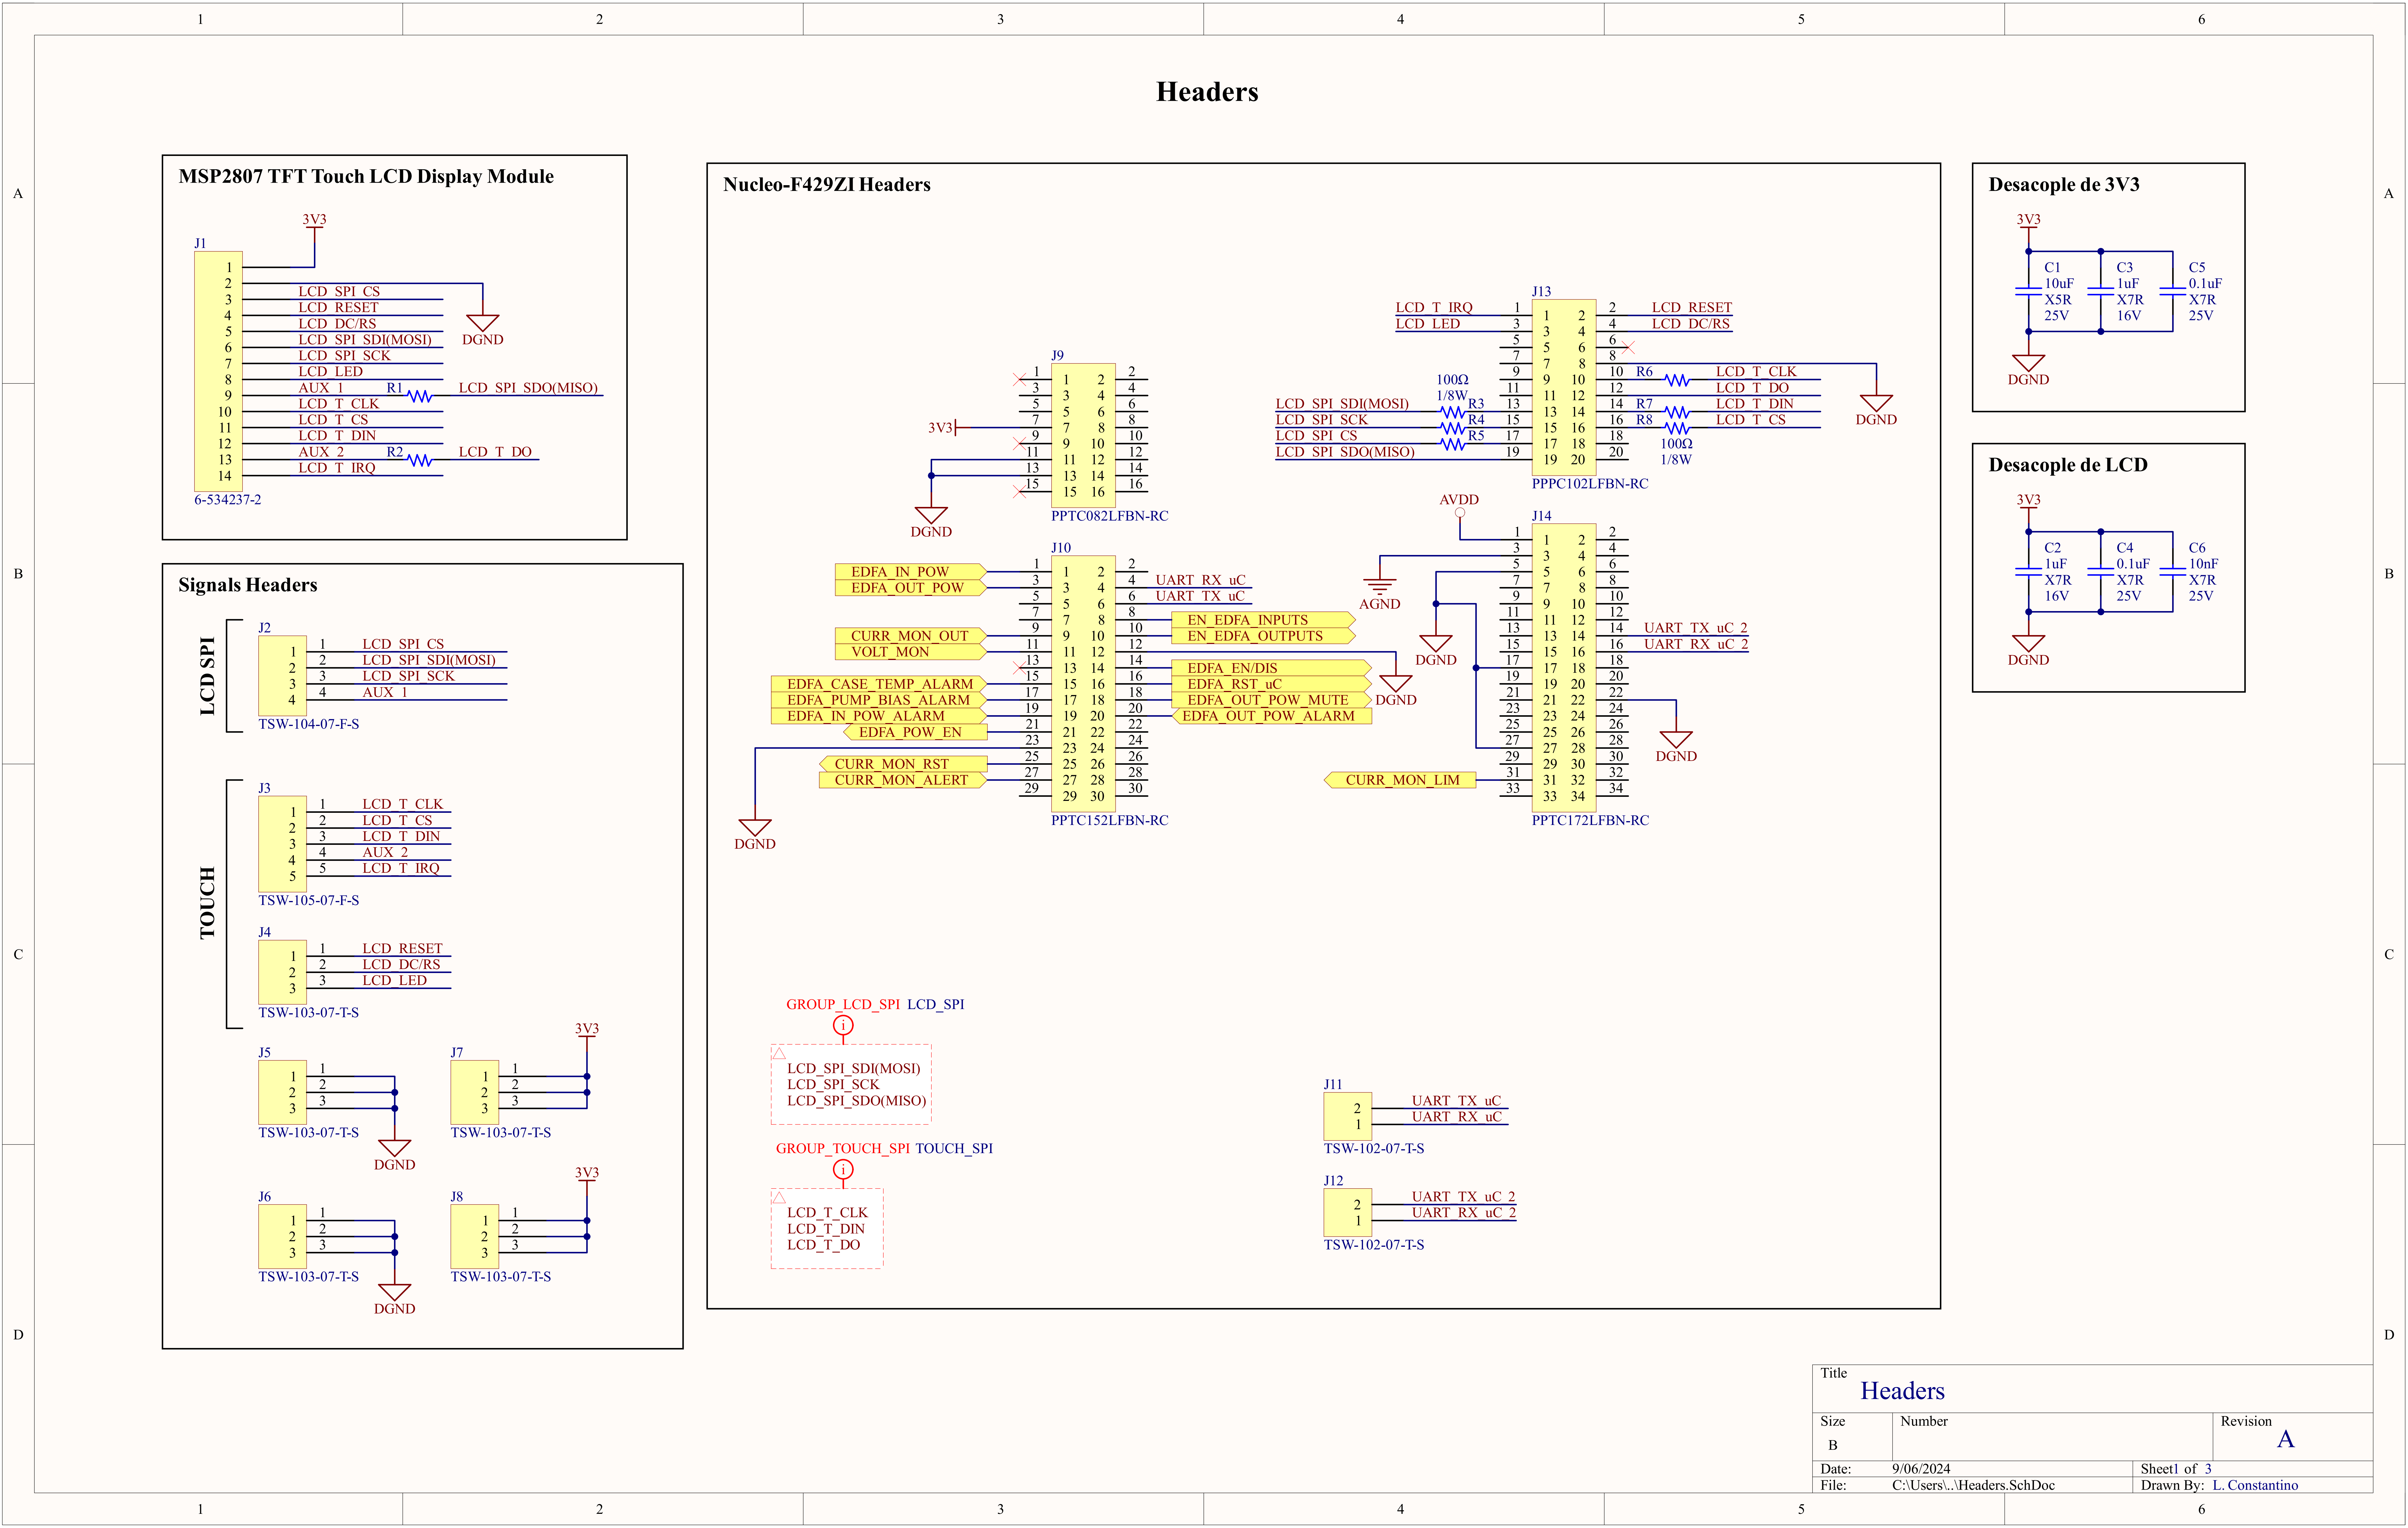
\includegraphics[width=1.7\textwidth]{./Figures/circ1.png}
\caption{Circuito esquemático. Conectores.}
\end{figure}

\begin{figure}[H]
\centering
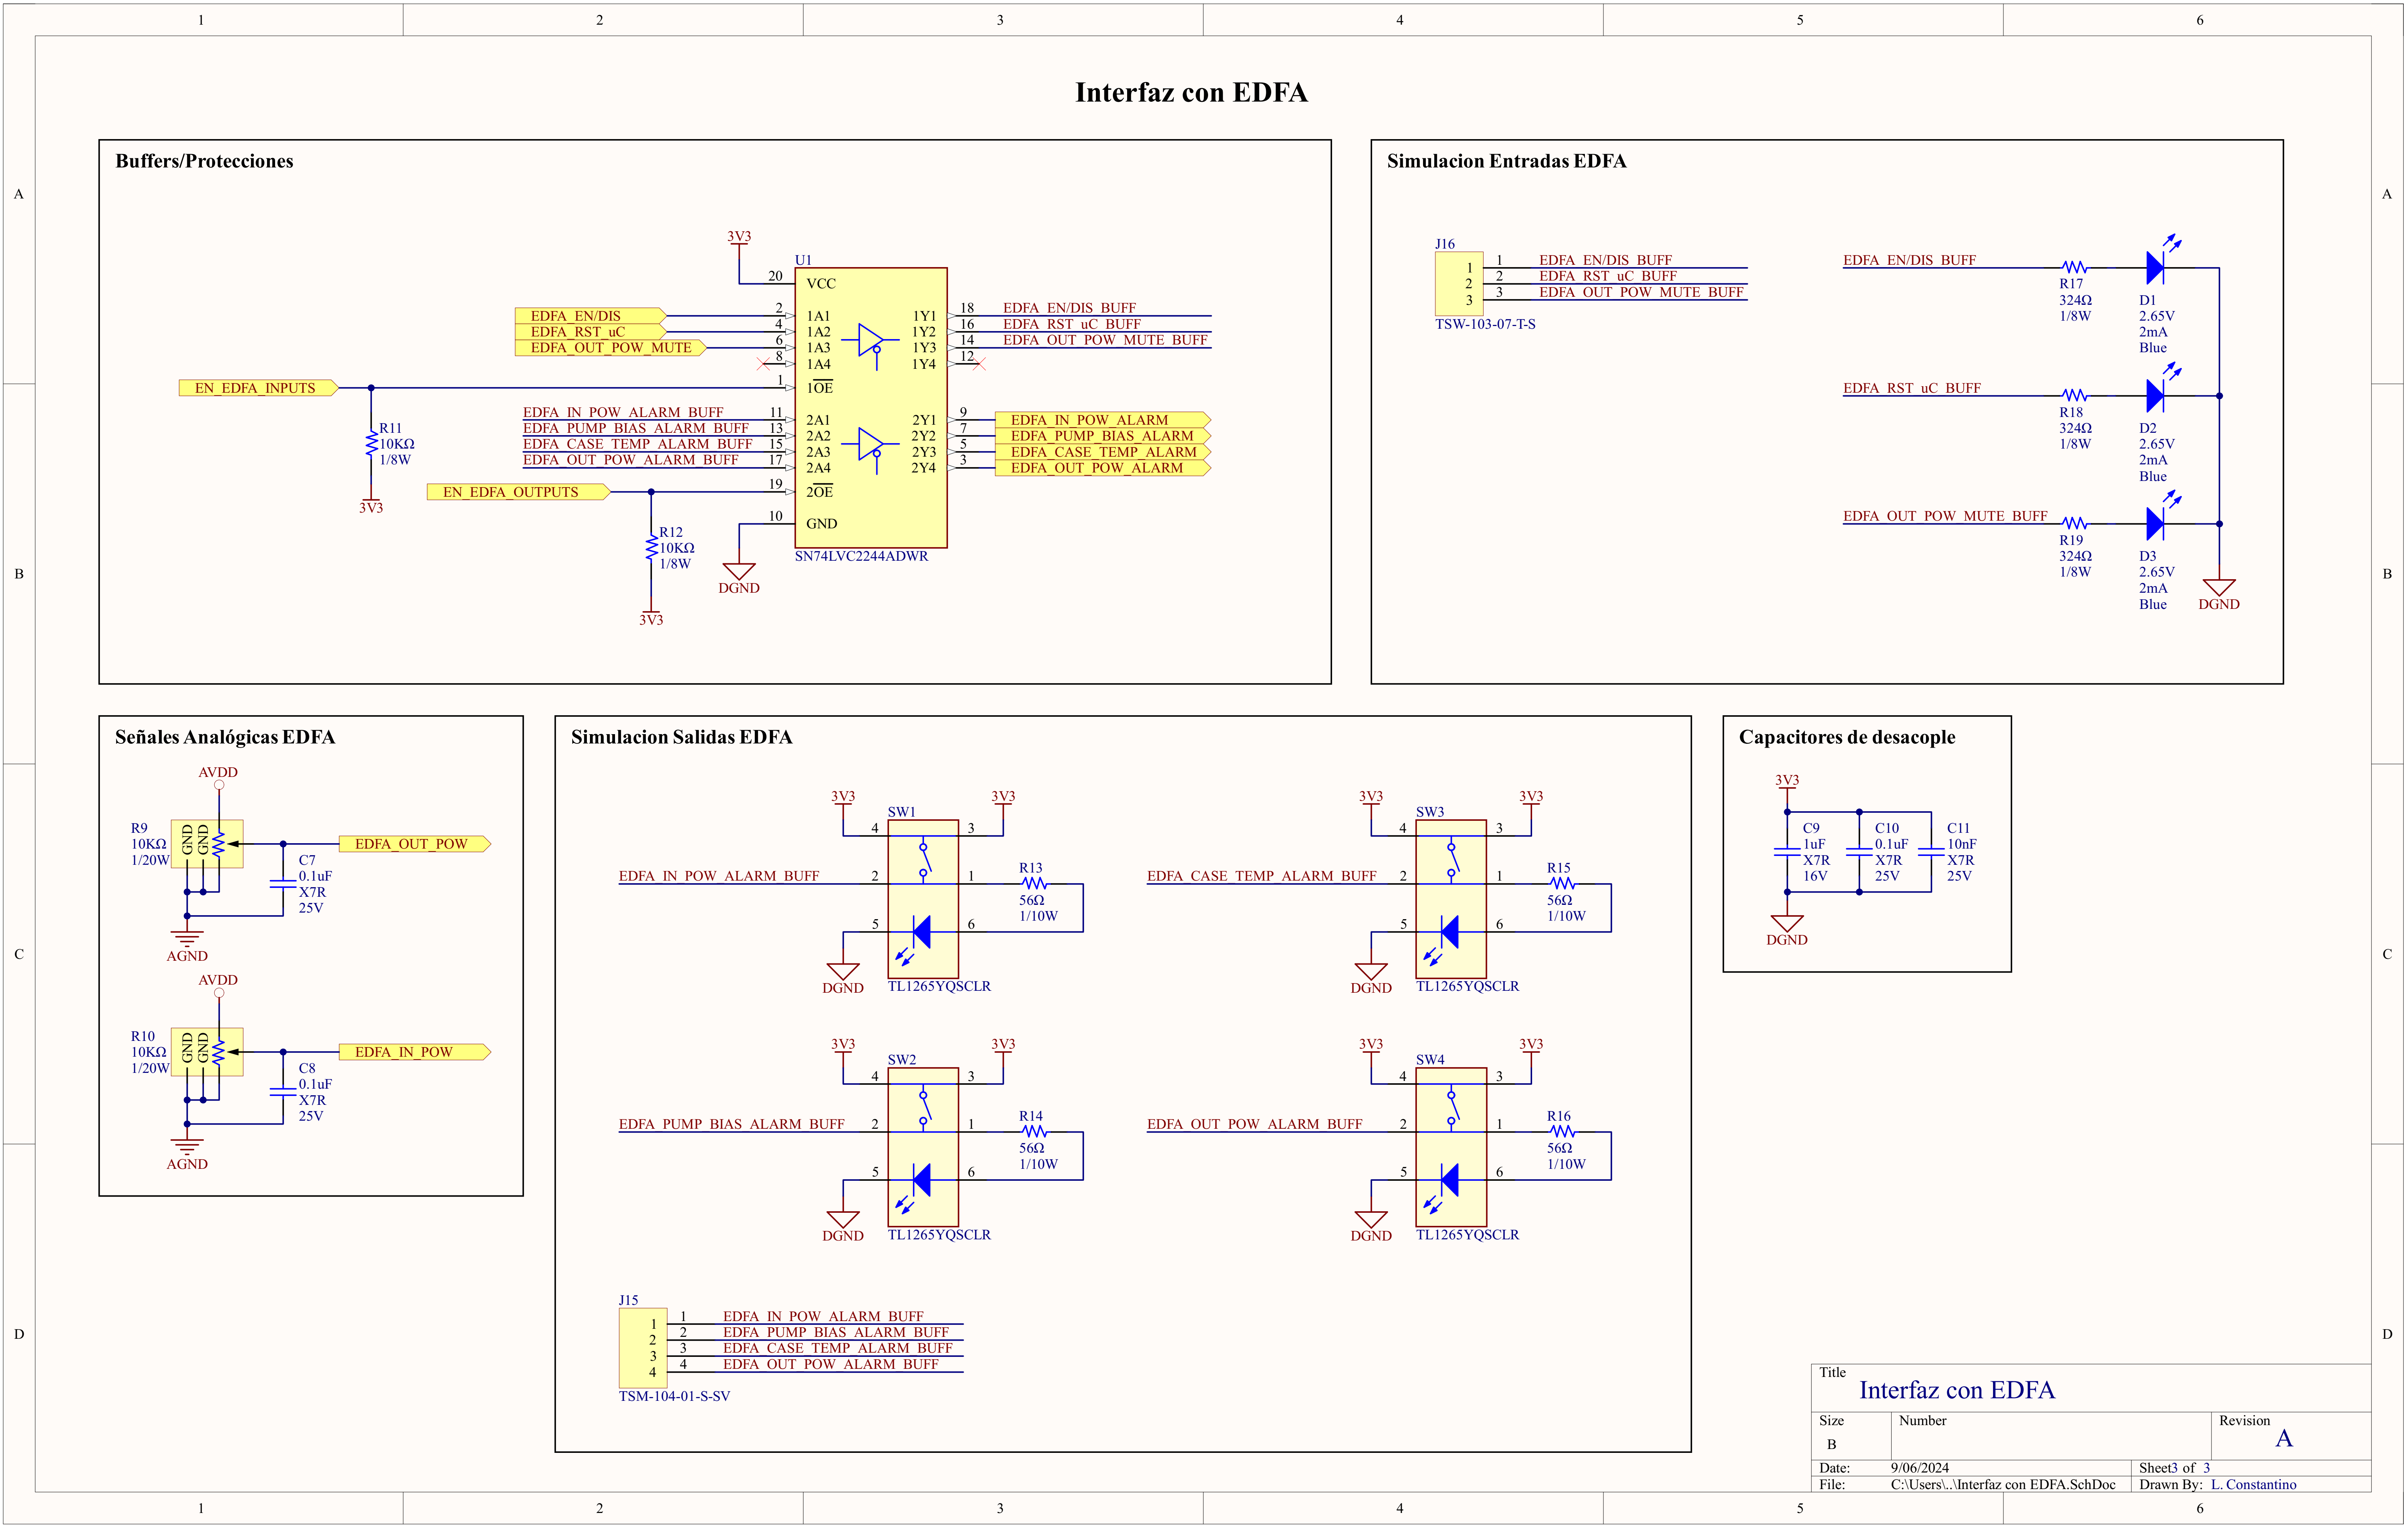
\includegraphics[width=1.7\textwidth]{./Figures/circ2.png}
\caption{Circuito esquemático. Interfaz con EDFA.}
\end{figure}

\begin{figure}[H]
\centering
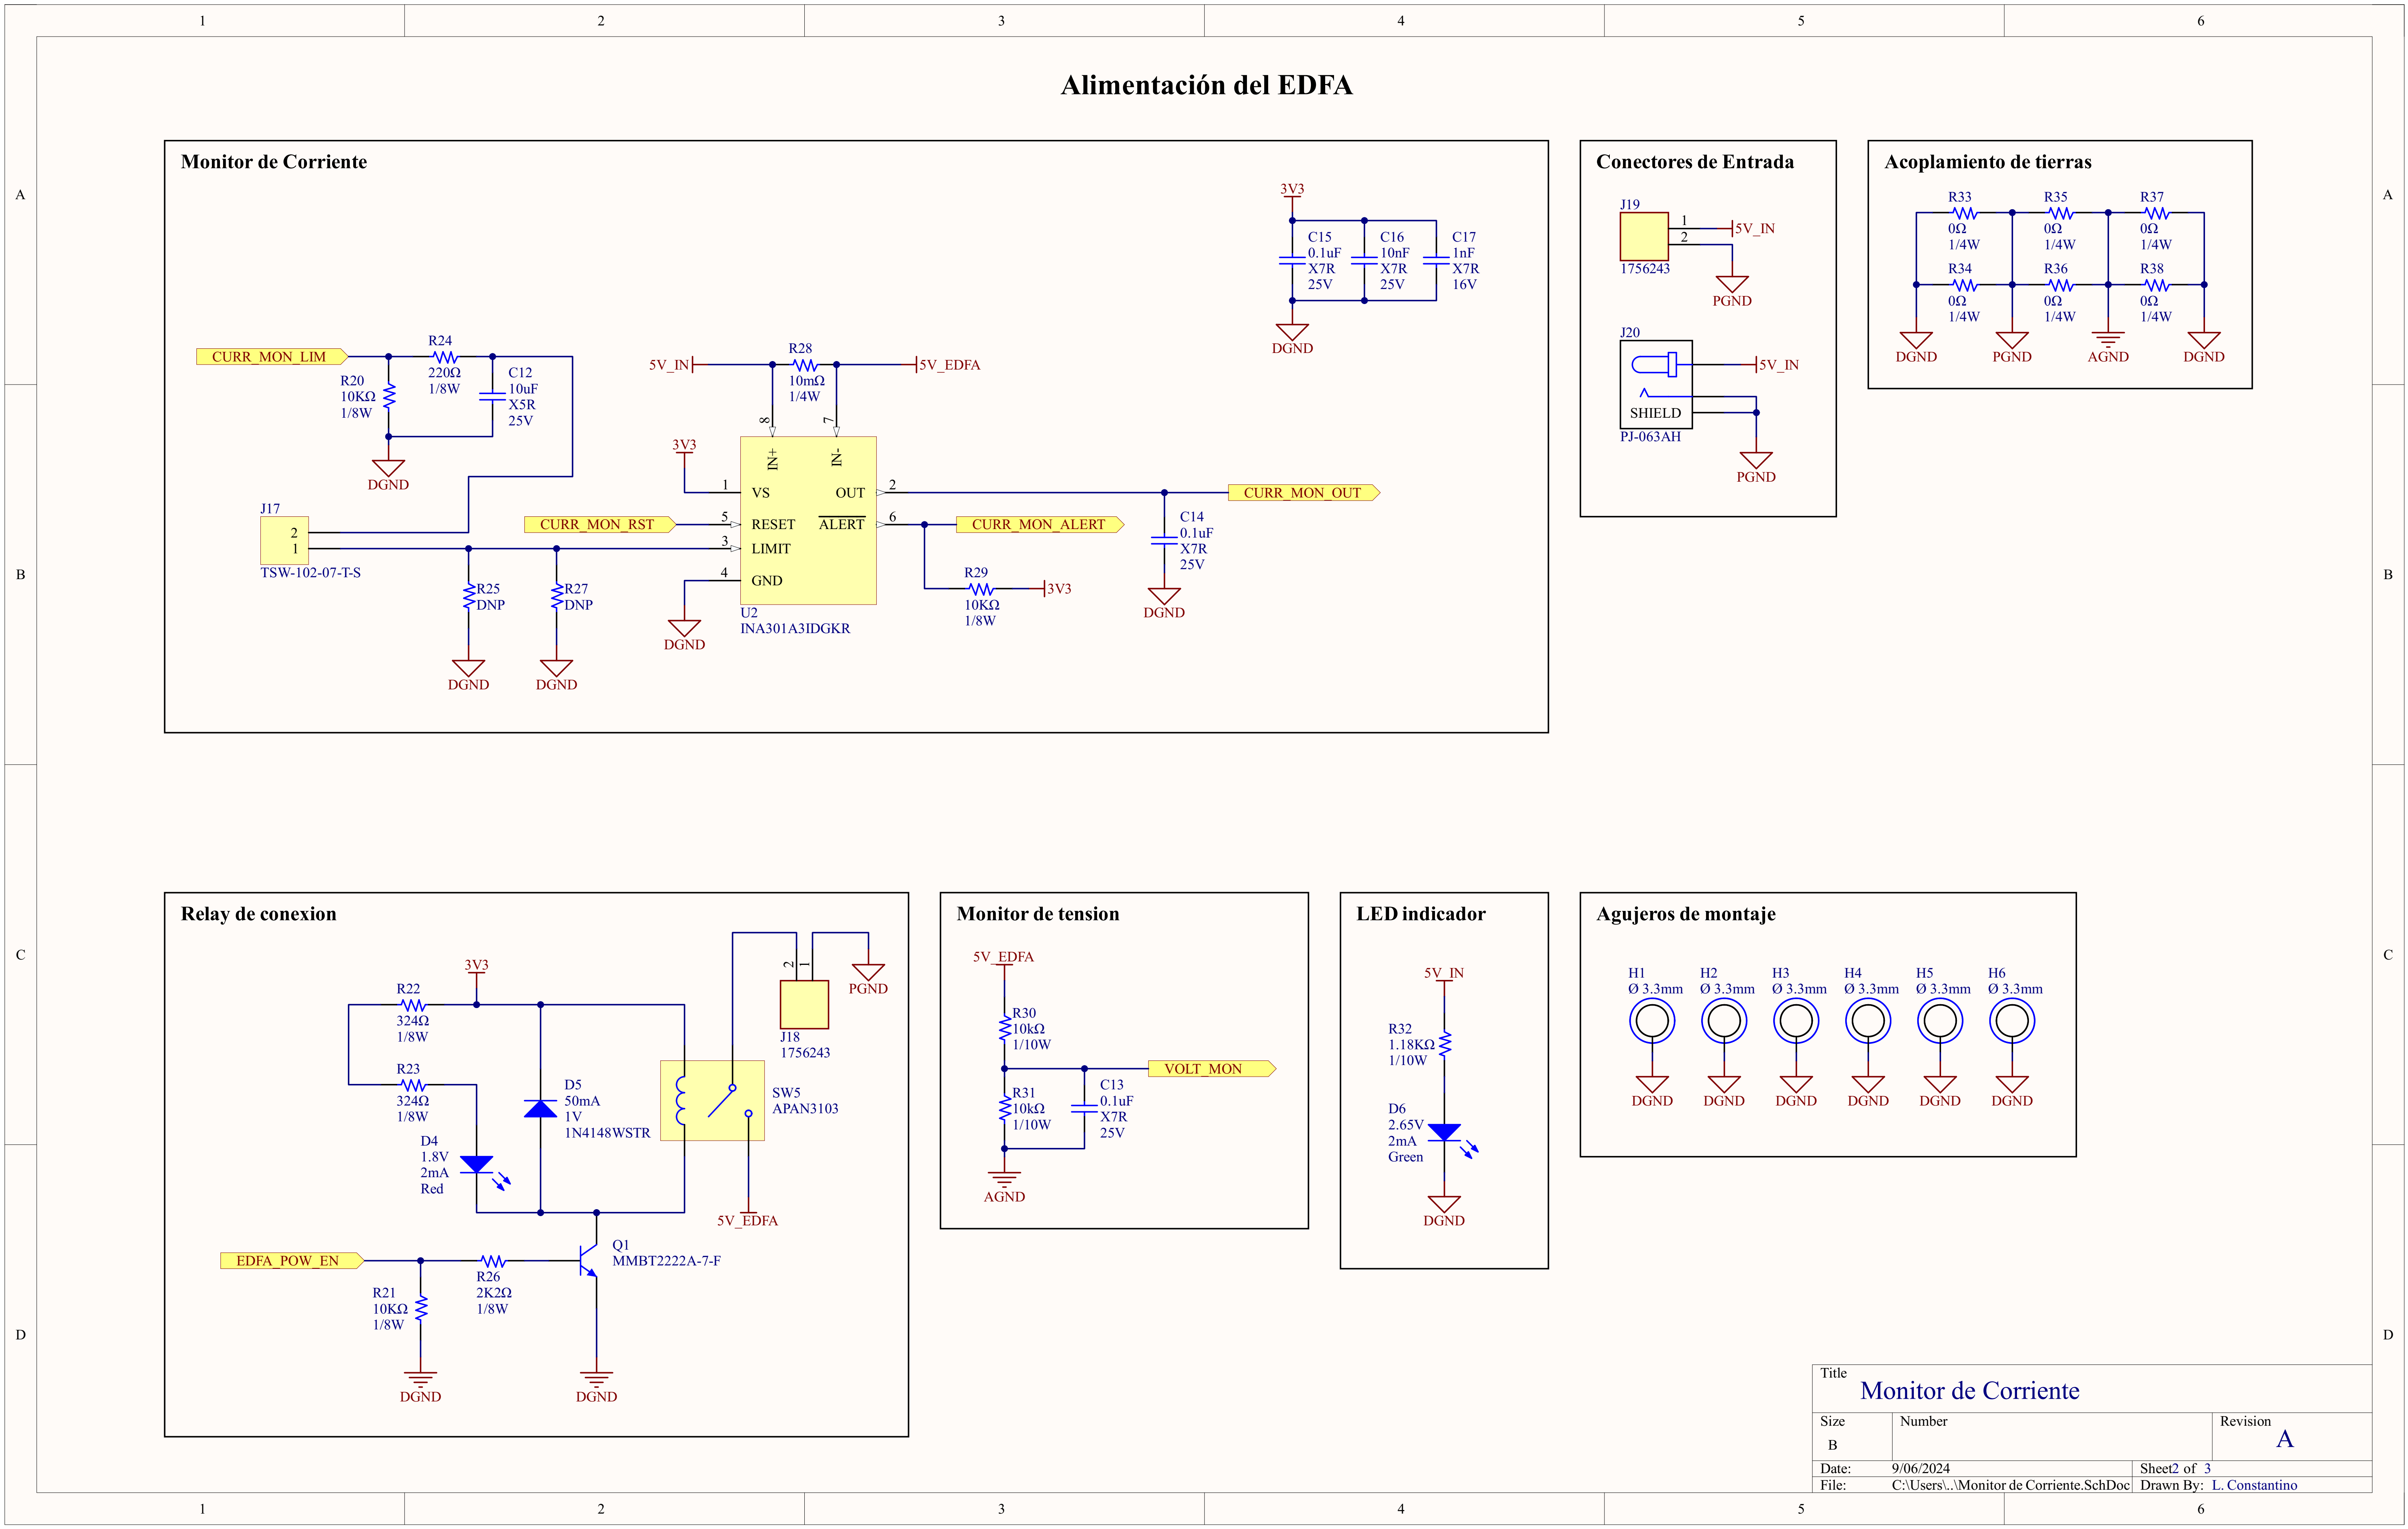
\includegraphics[width=1.7\textwidth]{./Figures/circ3.png}
\caption{Circuito esquemático. Alimentación del EDFA.}
\end{figure}
%% Appendix A

\chapter{Banco de ensayos} % Main appendix title

\label{AppendixB} % For referencing this appendix elsewhere, use \ref{AppendixA}

A continuación se puede ver el banco de ensayos con todos los instrumentos y componentes necesarios para ejecutar las pruebas de hardware y firmware.

\begin{figure}[H]
\centering
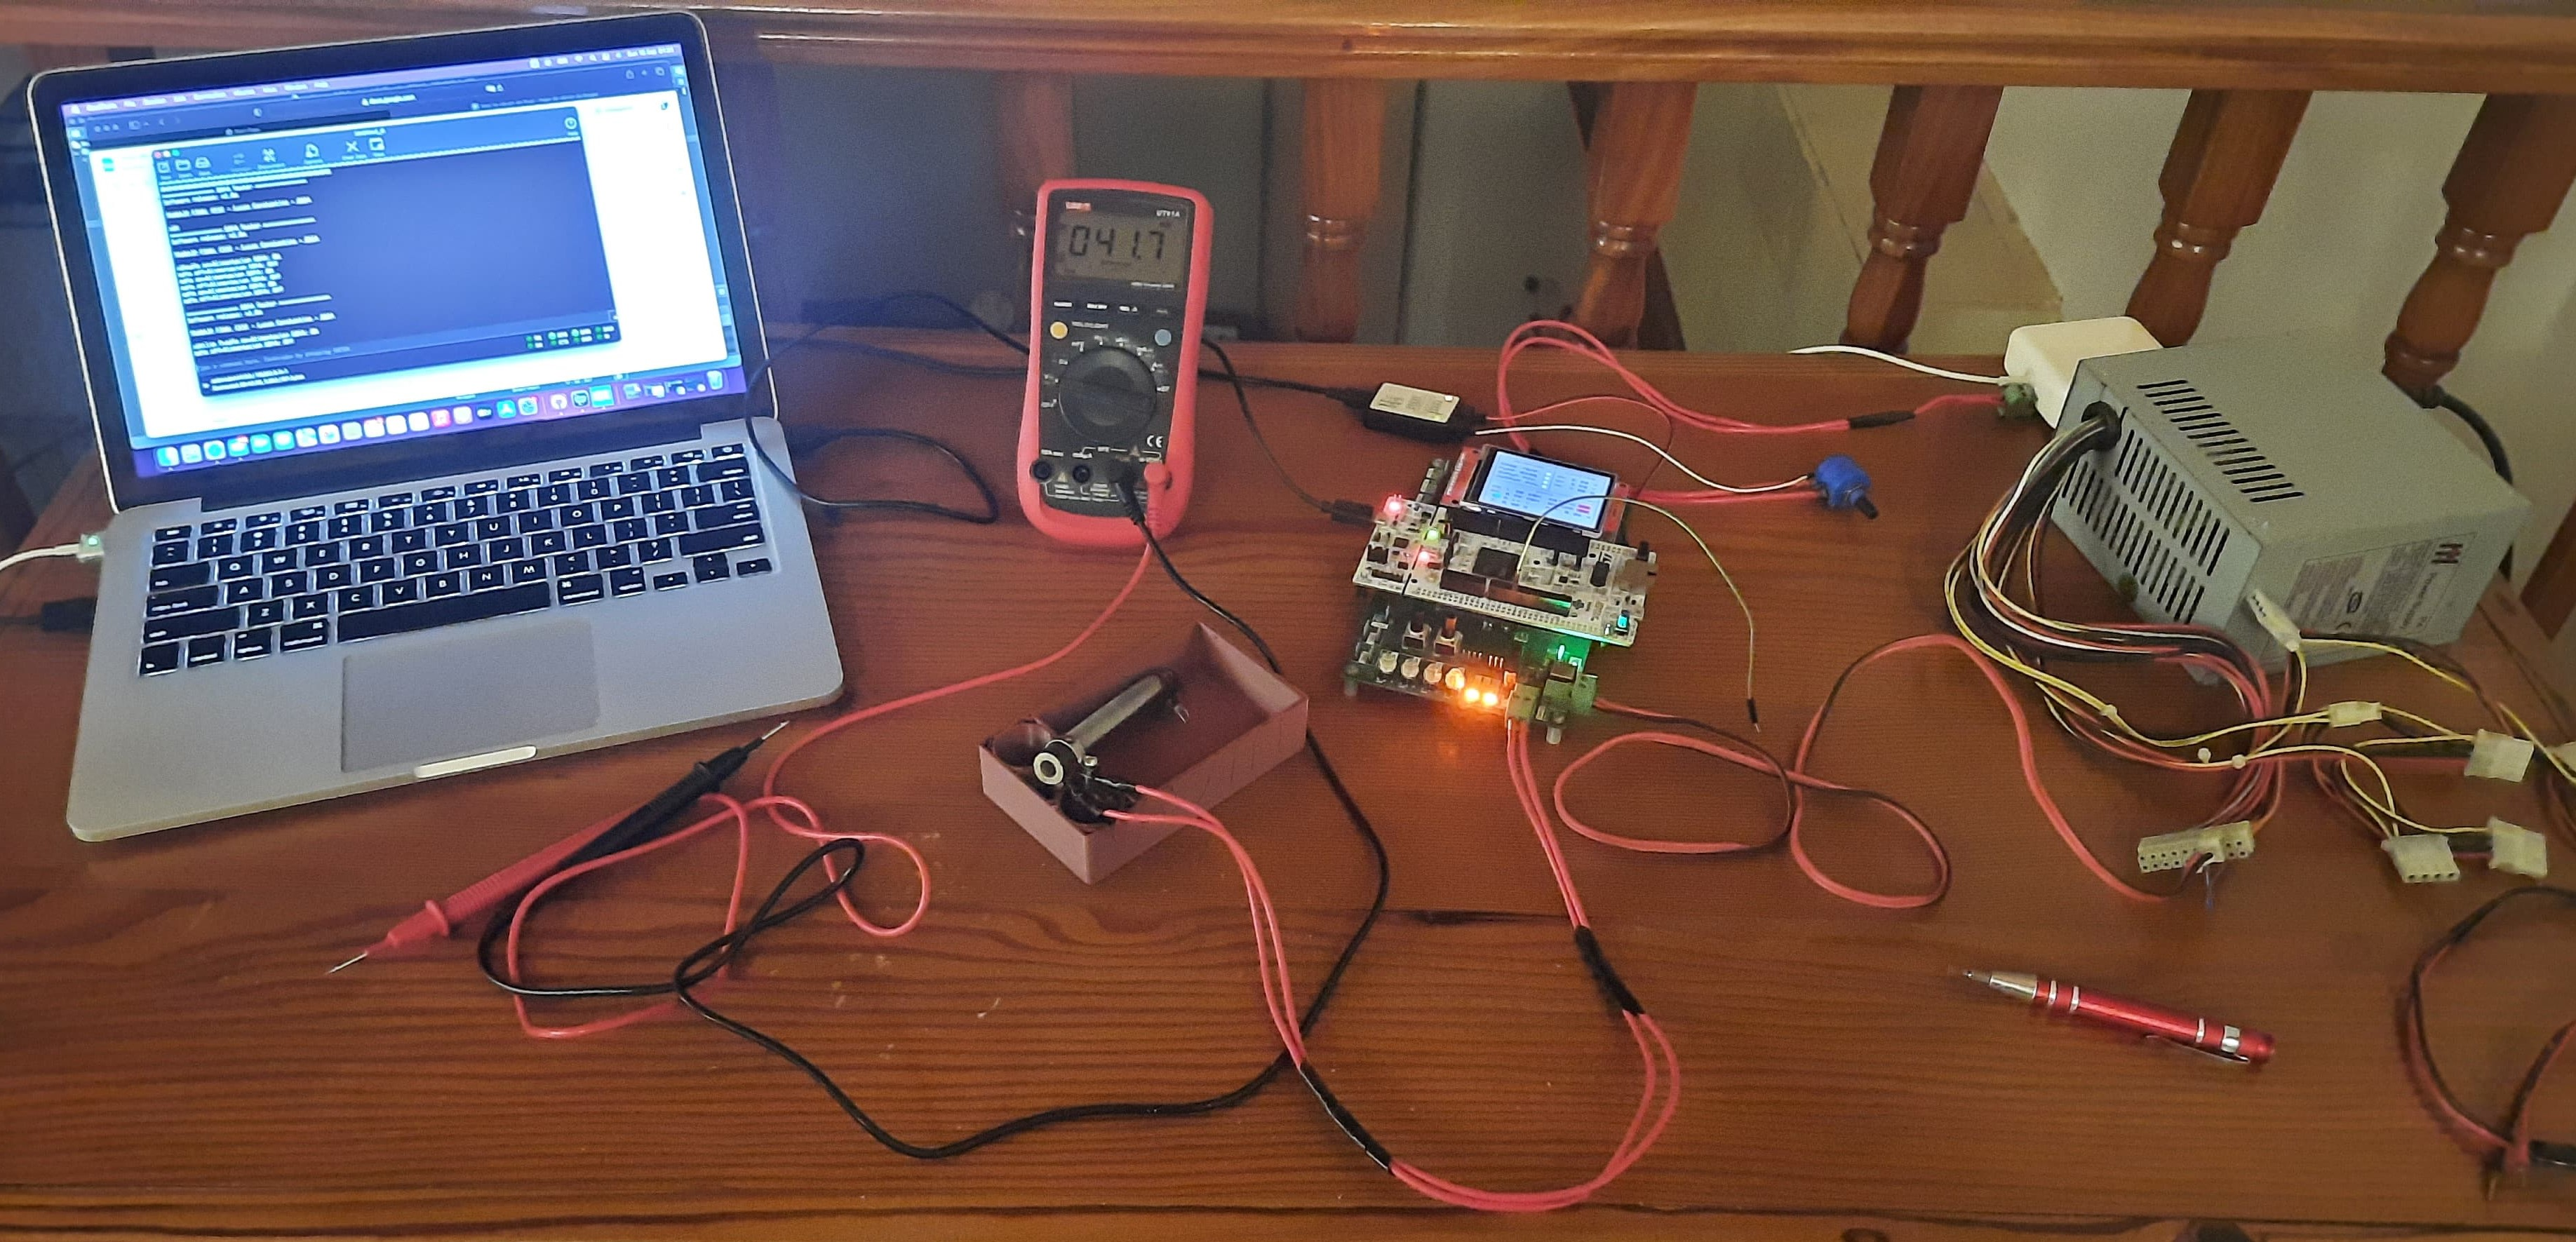
\includegraphics[width=1\textwidth]{./Figures/setupEnsayos.jpg}
\caption{Banco de ensayos.}
\label{fig:setupEnsayos}
\end{figure}
%\include{Appendices/AppendixC}

\end{landscape}

%----------------------------------------------------------------------------------------
%	BIBLIOGRAPHY
%----------------------------------------------------------------------------------------

\Urlmuskip=0mu plus 1mu\relax
\raggedright
\printbibliography[heading=bibintoc]

%----------------------------------------------------------------------------------------

\end{document}  
